%\documentclass{article}
%
%\usepackage{fancyhdr}
%\usepackage{extramarks}
%\usepackage{amsmath}
%\usepackage{amsthm}
%\usepackage{amsfonts}
%\usepackage{mathrsfs}
%\usepackage{tikz}
%\usepackage{enumerate}
%\usepackage{graphicx}
%\graphicspath{ {images/} }
%\usepackage[plain]{algorithm}
%\usepackage{algpseudocode}
%\usepackage[document]{ragged2e}
%\usepackage{textcomp}
%\usepackage{color}   %May be necessary if you want to color links
%\usepackage{import}
%\usepackage{hyperref}
%\hypersetup{
%    colorlinks=true, %set true if you want colored links
%    linktoc=all,     %set to all if you want both sections and subsections linked
%    linkcolor=black,  %choose some color if you want links to stand out
%}
%\usepackage{import}
%\usepackage{natbib}
%
%\usetikzlibrary{automata,positioning}
%
%
%% Basic Document Settings
%
%
%\topmargin=-0.45in
%\evensidemargin=0in
%\oddsidemargin=0in
%\textwidth=6.5in
%\textheight=9.0in
%\headsep=0.25in
%\setlength{\parskip}{1em}
%
%\linespread{1.1}
%
%\pagestyle{fancy}
%\lhead{\hmwkAuthorName}
%\lfoot{\lastxmark}
%\cfoot{\thepage}
%
%\renewcommand\headrulewidth{0.4pt}
%\renewcommand\footrulewidth{0.4pt}
%
%\setlength\parindent{0pt}
%
%
%\newcommand{\hmwkTitle}{Math Review Notes---Linear Regression}
%\newcommand{\hmwkAuthorName}{\textbf{G. Faletto} }
%
%
%% Title Page
%
%
%\title{
%    \vspace{2in}
%    \textmd{\textbf{ \hmwkTitle}}\\
%}
%
%\author{Gregory Faletto}
%\date{}
%
%\renewcommand{\part}[1]{\textbf{\large Part \Alph{partCounter}}\stepcounter{partCounter}\\}
%
%
%% Various Helper Commands
%
%
%% Useful for algorithms
%\newcommand{\alg}[1]{\textsc{\bfseries \footnotesize #1}}
%
%% For derivatives
%\newcommand{\deriv}[2]{\frac{\mathrm{d} #1}{\mathrm{d} #2}}
%
%% For partial derivatives
%\newcommand{\pderiv}[2]{\frac{\partial #1}{\partial #2}}
%
%% Integral dx
%\newcommand{\dx}{\mathrm{d}x}
%
%% Alias for the Solution section header
%\newcommand{\solution}{\textbf{\large Solution}}
%
% %Probability commands: Expectation, Variance, Covariance, Bias
%\newcommand{\E}{\mathbb{E}}
%\newcommand{\Var}{\mathrm{Var}}
%\newcommand{\Cov}{\mathrm{Cov}}
%\newcommand{\Bias}{\mathrm{Bias}}
%\newcommand\indep{\protect\mathpalette{\protect\independenT}{\perp}}
%\def\independenT#1#2{\mathrel{\rlap{$#1#2$}\mkern2mu{#1#2}}}
%\DeclareMathOperator{\Tr}{Tr}
%
%\theoremstyle{definition}
%\newtheorem{theorem}{Theorem}
%\theoremstyle{definition}
%\newtheorem{corollary}{Corollary}[theorem]
%\theoremstyle{definition}
%\newtheorem{proposition}[theorem]{Proposition}
%\theoremstyle{definition}
%\newtheorem{lemma}[theorem]{Lemma}
%\theoremstyle{definition}
%\newtheorem{definition}{Definition}[section]
%\newtheorem*{remark}{Remark}
%\theoremstyle{definition}
%\newtheorem{example}{Example}[section]
%
% %Tilde
%\newcommand{\textapprox}{\raisebox{0.5ex}{\texttildelow}}
%
%\begin{document}
%
%\maketitle
%
%\pagebreak
%
%\tableofcontents
%
%\
%
%\
%
%\begin{center}
%Last updated \today
%\end{center}
%
%
%
%\newpage
%
%%
%%
%%
%%
%%
%%
%%
%%
%
%% Econometrics and Linear Regression

\section{Linear Regression}

These notes are based on my notes from \textit{Time Series and Panel Data Econometrics} (1st edition) by M. Hashem Pesaran \citep{pesaran-2015-text} and coursework for Economics 613: Economic and Financial Time Series I at USC taught by M. Hashem Pesaran, DSO 607 at USC taught by Jinchi Lv, Statistics 100B at UCLA taught by Nicolas Christou, and the Coursera MOOC ``Econometrics: Methods and Applications" from Erasmus University Rotterdam. I also borrowed from some other sources which I mention when I use them.

%\section{Linear Regression}


%%%%%%%%%%% Linear Regression %%%%%%%%%%%%%
\subsection{Chapter 1: Linear Regression}

\subsubsection{Preliminaries}

Suppose the true model is \(y_i = \alpha + \beta x_i + \epsilon_i\). Classical assumptions:

\begin{enumerate}[(i)]

\item \(\E(\epsilon_i)= 0\)

\item \(\Var(\epsilon_i \mid x_i = \sigma^2\) (constant)

\item \(\Cov(\epsilon_i, \epsilon_j) = 0 \) if \(i \neq j\)

\item \(\epsilon_i\) is uncorrelated to \(x_i\), or \(\E(\epsilon_i \mid x_j) = 0 \) for all \(i, j\).

\end{enumerate}

\subsubsection{Estimation}

\[
\hat{\beta} = \frac{n\sum_{i=1}^n x_i y_i - \sum_{i=1}^n x_i \sum_{i=1}^n y_i}{n \sum_{i=1}^n x_i^2 - \big( \sum_{i=1}^n x_i \big)^2} = \frac{\sum_{i=1}^n x_i y_i - n \overline{x} \overline{y}}{\sum_{i=1}^n x_i^2 - n \overline{x}^2}
\]

\[
\hat{\alpha} = \overline{y} - \hat{\beta} \overline{x}
\]

or

\[
\hat{\beta} = \frac{\sum_{i=1}^n (x_i - \overline{x})(y_i - \overline{y})}{\sum_{i=1}^n(x_i - \overline{x})^2} = \frac{S_{XY}}{S_{XX}}
\]

or

\[
\hat{\beta} = r \frac{S_{YY}}{S_{XX}}
\]

where \(r\) is the correlation coefficient.

Let

\[
w_i = \frac{x_i - \overline{x}}{\sum_{i=1}^n (x_i - \overline{x})^2}
\]

so that 

\[
\hat{\beta} = \sum_{i=1}^n w_i( y_i - \overline{y}) = \sum_{i=1}^n w_i y_i  - \overline{y} \frac{  \sum_{i=1}^n x_i - \overline{x}}{\sum_{i=1}^n (x_i - \overline{x})^2} =  \sum_{i=1}^n w_i y_i 
\]

since \(  \sum_{i=1}^n x_i - \overline{x} = 0\). Then a simple expression for \(\Var(\hat{\beta})\) is 

\[
\Var(\hat{\beta}) = \sum_{i=1}^n w_i^2 \Var(y_i \mid x_i) = \sum_{i=1}^n w_i^2 \Var(\epsilon \mid x_i) = \sigma^2 \sum_{i=1}^n w_i^2 = \frac{\sigma^2}{\sum_{i=1}^n (x_i - \overline{x})^2} = \frac{\sigma^2}{S_{XX}}
\]

We can estimate these quantities as follows:

\[
\hat{\sigma}^2 = \frac{1}{n - 2} \cdot \sum_{i=1}^n(y_i - \hat{\alpha} - \hat{\beta} x_i)^2
\]

Note that

\[
\hat{\sigma}^2 =  \frac{1}{n - 2}\sum_{t=1}^T(y_t - \hat{\alpha} - \hat{\beta} x_t)^2 =  \frac{1}{n - 2}\sum_{t=1}^T \big[ (y_t - (\overline{y} - \hat{\beta} \overline{x}) - \hat{\beta} x_t)^2 \big] = \frac{1}{n - 2} \sum_{t=1}^T(y_t - \overline{y} - \hat{\beta}( x_t - \overline{x}))^2 
\]

\[
=\frac{1}{n - 2} \sum_{t=1}^T(y_t - \overline{y})^2 - 2\hat{\beta}( x_t - \overline{x})(y_t - \overline{y})+ \hat{\beta}^2( x_t - \overline{x})^2
\]

In the case where there is no intercept, we have

\[
\hat{\sigma}^2 =  \frac{1}{T - 1}\sum_{t=1}^T(y_t  - \hat{\beta} x_t)^2 = \frac{1}{T - 1} \sum_{t=1}^T \bigg(y_t^2 - 2r \frac{S_{YY}}{S_{XX}}x_ty_t + r^2 \frac{S_{YY}^2}{S_{XX}^2} x_t^2 \bigg)
\]

Also,

\[
\widehat{\Var}(\hat{\beta}) = \frac{\hat{\sigma}^2}{S_{XX}} = \frac{1}{n - 2} \cdot \frac{ \sum_{i=1}^n(y_i - \hat{\alpha} - \hat{\beta} x_i)^2 }{\sum_{i=1}^n (x_i - \overline{x})^2 }
\]

Correlation coefficient:

\[
r^2 =  \frac{\big(\sum_{t=1}^T x_t y_t \big)^2}{\sum_{t=1}^T x_t^2 \sum_{t=1}^T y_t^2 }
\]

\[
r = \frac{1}{T-1} \frac{S_{XY}}{\sqrt{S_{XX}S_{YY}}}
\]

\begin{remark}The formulas for the coefficients in univariate OLS can also be derived by considering \((x, y)\) as a bivariate normal distribution and calculating the conditional expectation of \(y\) given \(x\). (See Proposition (\ref{prob.cond.bivar.norm.dist}).)\end{remark}

\begin{proposition}[\textbf{Stats 100B homework problem}] Consider the regression model \(y_i = \beta_0 + \beta_1 x_i + \epsilon_i\) with \(x_i\) fixed and \(\epsilon_i \sim \mathcal{N}(0, \sigma^2)\), \(\epsilon_i\) i.i.d. Let \(e_i = y_i - \hat{y}_i\) be the residuals.

\begin{enumerate}[(a)]

\item 

\[
\sum_{i=1}^n e_i = 0
\]

\item \(\Cov(\overline{Y}, \hat{\beta}_1) =0\) where \(\overline{Y}\) is the sample mean of the \(y\) values.


\item 

\[
\Cov(e_i, e_j)  = \sigma^2\bigg(-\frac{1}{n} - \frac{ (x_i -\bar{x})(x_j - \bar{x})}{\sum_{k=1}^n(x_k - \bar{x})^2} \bigg)
\]

\item We can construct a confidence interval for \(\sigma^2\) as 

\[
 \Pr \bigg( \frac{\sum_{i=1}^n e_i^2}{\chi_{1 - \frac{\alpha}{2}; n-2}^2}  \leq \sigma^2  \leq  \frac{\sum_{i=1}^n e_i^2}{\chi_{\frac{\alpha}{2}; n-2}^2}  \bigg) = 1 - \alpha 
\]

\end{enumerate}

\end{proposition}

\begin{proof}

\begin{enumerate}[(a)]

\item \[
\sum_{i=1}^n e_i = \sum_{i=1}^n(y_i - \hat{y}_i) = \sum_{i=1}^n(y_i - [\bar{y} + \hat{\beta_1}(x_i - \bar{x})])
\]

\[
= \sum_{i=1}^n\bigg(y_i - \bar{y} - \frac{\sum(x_i - \bar{x}) y_i}{\sum(x_i - \bar{x})^2}(x_i - \bar{x})\bigg)  = \sum_{i=1}^n y_i - n\bar{y} - \frac{\sum(x_i - \bar{x}) y_i}{\sum(x_i - \bar{x})^2} \sum_{i=1}^n (x_i - \bar{x})
\]

\[
= \sum_{i=1}^n y_i - n \frac{1}{n} \sum_{i=1}^n y_i - \bigg( \frac{\sum(x_i -  \bar{x}) y_i}{\sum(x_i - \bar{x})^2} \bigg) \bigg[ \sum_{i=1}^n \bigg( x_i - \frac{1}{n}\sum_{i=1}^n x_i \bigg)\bigg]
\]

\[
= \sum_{i=1}^n (y_i - y_i)  - \bigg( \frac{\sum(x_i -  \bar{x}) y_i}{\sum(x_i - \bar{x})^2} \bigg) \bigg[ \sum_{i=1}^n x_i - \frac{1}{n} \cdot n\sum_{i=1}^n x_i\bigg] = 0 - 0 = \boxed{0}
\]

Or:

\[
\sum_{i=1}^n e_i = \sum_{i=1}^n(y_i - \hat{y}_i) = \sum_{i=1}^n(y_i - \hat{\beta_0} - \hat{\beta_1}x_i) = \sum_{i=1}^n(y_i - (\bar{y} - \hat{\beta_1} \bar{x}) - \hat{\beta_1}x_i) 
\]

\[
= \sum_{i=1}^n(y_i - \bar{y})  - \hat{\beta_1}\sum_{i=1}^n( x_i - \bar{x})  = 0
\]


\item \[
\Cov(\bar{Y}, \hat{\beta_1}) = \Cov\bigg(\frac{1}{n} \sum_{i=1}^n Y_i , \frac{\sum_{i=1}^n (x_i - \bar{x})Y_i}{\sum_{i=1}^n (x_i - \bar{x})^2} \bigg) = \frac{1}{n\sum_{i=1}^n (x_i - \bar{x})^2}\Cov\bigg( \sum_{i=1}^n Y_i , \sum_{i=1}^n (x_i - \bar{x})Y_i\bigg)
\]

\(x_i\) is fixed, \(\Cov(Y_i, Y_j) = 0 \) for \(i \neq j\) by assumption of the model, \(\Var(Y_i) = \sigma^2\) by assumption of the model. 

\[
= \frac{1}{n\sum_{i=1}^n (x_i - \bar{x})^2} \sum_{i=1}^n[(x_i - \bar{x})  \Var ( Y_i)  ] = \frac{\sigma^2}{n\sum_{i=1}^n (x_i - \bar{x})^2} \sum_{i=1}^n(x_i - \bar{x})   = \boxed{0}
\]

\item \[
\Cov(e_i, e_j) = \Cov(y_i - \bar{y} - \hat{\beta_1}(x_i - \bar{x}), y_j - \bar{y} - \hat{\beta_1}(x_j - \bar{x}))
\]

\[
 = \Cov(y_i, y_j) - \Cov(y_i, \bar{y}) - \Cov(y_i, \hat{\beta_1}(x_j - \bar{x})) - \Cov(\bar{y}, y_j)  + \Cov(\bar{y}, \bar{y}) + \Cov(\bar{y}, \hat{\beta_1}(x_j - \bar{x})) - \Cov(\hat{\beta_1}(x_i - \bar{x}), y_j) 
\]

\[
+ \Cov(\hat{\beta_1}(x_i - \bar{x}), \bar{y}) + \Cov(\hat{\beta_1}(x_i - \bar{x}), \hat{\beta_1}(x_j - \bar{x}))
\]

By assumption of the model, \(\Cov(y_i, y_j) = 0\). 

\[
 = 0 - \Cov(y_i, \bar{y}) - ( x_j - \bar{x} )\Cov(y_i, \hat{\beta_1} )  - \Cov(\bar{y}, y_j)  + \Var(\bar{y}) + (x_j - \bar{x}) \Cov(\bar{y}, \hat{\beta_1}) -  (x_i - \bar{x}) \Cov(\hat{\beta_1}, y_j)   
\]

\[
+ (x_i  - \bar{x}) \Cov(\hat{\beta_1} , \bar{y} ) + (x_i - \bar{x})(x_j - \bar{x})\Cov(\hat{\beta_1}, \hat{\beta_1})
\]


In part 7(b) we showed \( \Cov(\bar{y}, \hat{\beta_1}) = 0 \). \(\Var(\bar{y}) = \sigma^2/n\). \(\Cov(\hat{\beta_1}, \hat{\beta_1}) = \Var(\hat{\beta_1}) = \sigma^2/\sum(x_k - \bar{x})^2\). So this simplifies to 

\[
 = - \Cov(y_i, \bar{y}) - ( x_j - \bar{x})\Cov(y_i, \hat{\beta_1} ) - \Cov(y_j, \bar{y}) + \frac{\sigma^2}{n} + 0 - ( x_i - \bar{x})\Cov(y_j, \hat{\beta_1} ) + 0 + (x_i - \bar{x})(x_j - \bar{x})\frac{\sigma^2}{\sum_{k=1}^n(x_k - \bar{x})^2}
\]

\begin{equation} \label{linreg.100b.hw5.8}
 =- \Cov(y_i, \bar{y}) - ( x_j - \bar{x})\Cov(y_i, \hat{\beta_1} ) - \Cov(y_j, \bar{y}) + \frac{\sigma^2}{n} - ( x_i - \bar{x})\Cov(y_j, \hat{\beta_1} ) + (x_i - \bar{x})(x_j - \bar{x})\frac{\sigma^2}{\sum_{k=1}^n(x_k - \bar{x})^2}
\end{equation}

Find \(\Cov(y_i, \bar{y}), \Cov(y_j, \bar{y}), \Cov(y_i, \hat{\beta_1} ), \) and \(\Cov(y_j, \hat{\beta_1} )\):

%\begin{center}
%\noindent\rule{12cm}{0.4pt}
%\end{center}

%\vspace{1em}

%\textbf{Easy way} 

Using that \(x_i\) is fixed, \(\Cov(Y_i, Y_j) = 0 \) for \(i \neq j\) by assumption of the model, \(\Var(Y_i) = \sigma^2\) by assumption of the model:

\[
\Cov(y_i, \bar{y}) = \Cov\bigg(y_i, \frac{1}{n}\sum_{k=1}^n y_k  \bigg) = \frac{1}{n} \Cov(y_i, y_i) = \frac{\sigma^2}{n}
\]

Similarly, 

\[
\Cov(y_j, \bar{y})  = \frac{\sigma^2}{n}
\]

\[
\Cov(y_i, \hat{\beta_1}) = \Cov \bigg(y_i, \frac{\sum_{k=1}^n (x_k - \bar{x})y_i}{\sum_{k=1}^n (x_k - \bar{x})^2} \bigg) = \frac{1}{\sum_{k=1}^n (x_k - \bar{x})^2} \Cov \bigg(y_i, \sum_{k=1}^n (x_k - \bar{x})y_i \bigg)
\]

\[
= \frac{1}{\sum_{k=1}^n (x_k - \bar{x})^2} \Cov (y_i,  (x_i - \bar{x})y_i ) = \frac{x_i - \bar{x}}{\sum_{k=1}^n (x_k - \bar{x})^2} \Var (y_i) = \frac{x_i - \bar{x}}{\sum_{k=1}^n (x_k - \bar{x})^2}  \sigma^2
\]

Similarly, 

\[
\Cov(y_j, \hat{\beta_1}) = \frac{x_j - \bar{x}}{\sum_{k=1}^n (x_k - \bar{x})^2}  \sigma^2
\]

%\textbf{Hard way:} Find a matrix \(\boldsymbol{A}\) such that \(\boldsymbol{A}\vec{Y} = \begin{pmatrix} \vec{Y} \ \bar{Y} \ \hat{\beta_1} \end{pmatrix}' \). Then the covariance matrix \(\Var(\boldsymbol{A}\vec{Y}) = \boldsymbol{A} \Var(\vec{Y}) \boldsymbol{A}' = \boldsymbol{A} (\sigma^2 \boldsymbol{I}) \boldsymbol{A}' = \sigma^2 \boldsymbol{A} \boldsymbol{A}'\) will contain \(\Cov(y_i, \bar{y}), \Cov(y_j, \bar{y}), \Cov(y_i, \hat{\beta_1} ), \) and \(\Cov(y_j, \hat{\beta_1} )\). 
%
%%\vspace{1em}
%%
%%(Note: Since \(\boldsymbol{A}\vec{Y}\) is multivariate normal, if  \(\Cov(\bar{Y}, \hat{\beta_1}) = 0 \) then \(\bar{Y}\) and \(\hat{\beta_1}\) are independent.)
%
%\[
%\boxed{
%\bar{Y} = \frac{1}{n} \boldsymbol{1}'\vec{Y}}
%\]
%
%\[
%\hat{\beta_1} = \frac{\sum(x_k - \bar{x}) y_k}{\sum(x_k - \bar{x})^2}
%\]
%
%\[
%\boxed{
%\hat{\beta_1} = \frac{\boldsymbol{q}' }{\boldsymbol{q}'\boldsymbol{q}} \vec{Y}}
%\]
%
%(defining \(\boldsymbol{q}\) as in question 7(b). Therefore 
%
%\[
%\begin{pmatrix}
%\boldsymbol{I} \\
%\frac{1}{n} \boldsymbol{1}' \\
%\frac{\boldsymbol{q}' }{\boldsymbol{q}'\boldsymbol{q}}
%\end{pmatrix} \vec{Y} = \begin{pmatrix}
%\vec{Y} \\
%\bar{Y} \\
%\hat{\beta_1} 
%\end{pmatrix}
%\]
%
%So
%
%\[
%\boldsymbol{A} = \begin{pmatrix}
%\boldsymbol{I} \\
%\frac{1}{n} \boldsymbol{1}' \\
%\frac{\boldsymbol{q}' }{\boldsymbol{q}'\boldsymbol{q}}
%\end{pmatrix} 
%\]
%
%To find the variance matrix, we calculate
%
%\[
%\sigma^2 \boldsymbol{A} \boldsymbol{A}' = \sigma^2 \begin{pmatrix}
%\boldsymbol{I} \\
%\frac{1}{n} \boldsymbol{1}' \\
%\frac{\boldsymbol{q}' }{\boldsymbol{q}'\boldsymbol{q}}
%\end{pmatrix} \begin{pmatrix}
%\boldsymbol{I} \ \frac{1}{n} \boldsymbol{1} \ \frac{\boldsymbol{q} }{\boldsymbol{q}'\boldsymbol{q}}
%\end{pmatrix} = \sigma^2 \begin{pmatrix}
%\boldsymbol{I} \ \frac{1}{n} \boldsymbol{1} \ \frac{\boldsymbol{q} }{\boldsymbol{q}'\boldsymbol{q}} \\
%\frac{1}{n} \boldsymbol{1}'  \ \frac{1}{n^2}\boldsymbol{1}'\boldsymbol{1} \ \frac{1}{n\boldsymbol{q}'\boldsymbol{q}} \boldsymbol{1}'\boldsymbol{q} \\
%\frac{\boldsymbol{q}' }{\boldsymbol{q}'\boldsymbol{q}} \ \frac{1}{n \boldsymbol{q}'\boldsymbol{q}} \boldsymbol{q}' \boldsymbol{1} \ \frac{1}{(\boldsymbol{q}'\boldsymbol{q})^2} \boldsymbol{q}'\boldsymbol{q}
%\end{pmatrix} = \sigma^2 \begin{pmatrix}
%\boldsymbol{I} \ \frac{1}{n} \boldsymbol{1} \ \frac{\boldsymbol{q} }{\boldsymbol{q}'\boldsymbol{q}} \\
%\frac{1}{n} \boldsymbol{1}'  \  \frac{n}{n^2} \ \frac{1}{n\boldsymbol{q}'\boldsymbol{q}} \boldsymbol{1}'\boldsymbol{q} \\
%\frac{\boldsymbol{q}' }{\boldsymbol{q}'\boldsymbol{q}} \  \frac{1}{n \boldsymbol{q}'\boldsymbol{q}} \boldsymbol{q}' \boldsymbol{1} \ \frac{1}{\boldsymbol{q}'\boldsymbol{q}}
%\end{pmatrix}
%\]
%
%But
%
%\[
%\boldsymbol{1}'\boldsymbol{q}  = \boldsymbol{q}' \boldsymbol{1} = \sum_{i=1}^n (x_i - \bar{x}) = \sum_{i=1}^n \bigg( x_i - \frac{1}{n}\sum_{j=1}^n x_j \bigg) = \sum_{i=1}^n x_i - \frac{1}{n} \cdot n\sum_{j=1}^n x_j = 0
%\]
%
%So we have 
% 
%\[
%\Var(\boldsymbol{A}\vec{Y}) = \sigma^2 \boldsymbol{A} \boldsymbol{A}' = \sigma^2 \begin{pmatrix}
%\boldsymbol{I} \ \frac{1}{n} \boldsymbol{1} \ \frac{\boldsymbol{q} }{\boldsymbol{q}'\boldsymbol{q}} \\
%\frac{1}{n} \boldsymbol{1}'  \  \frac{1}{n} \ 0 \\
%\frac{\boldsymbol{q}' }{\boldsymbol{q}'\boldsymbol{q}} \  0 \ \frac{1}{\boldsymbol{q}'\boldsymbol{q}}
%\end{pmatrix}
%\]
%
%This implies
%
%\[
%\Cov(y_i, \bar{y}) = \Cov(y_j, \bar{y}) = \frac{\sigma^2}{n}
%\]
%
%and 
%
%\[
%\Cov(y_i, \hat{\beta_1}) = \frac{(x_i - \bar{x})\sigma^2}{\sum_{k=1}^n(x_k - \bar{x})^2}, \Cov(y_j, \hat{\beta_1}) = \frac{(x_j - \bar{x})\sigma^2}{\sum_{k=1}^n(x_k - \bar{x})^2}
%\]
%
%\begin{center}
%\noindent\rule{12cm}{0.4pt}
%\end{center}

Plugging these in to equation (\ref{linreg.100b.hw5.8}) yields


\[
\Cov(e_i, e_j)  = -\frac{\sigma^2}{n} - ( x_j - \bar{x})\frac{(x_i - \bar{x})\sigma^2}{\sum_{k=1}^n(x_k - \bar{x})^2} -\frac{\sigma^2}{n} + \frac{\sigma^2}{n}  - ( x_i - \bar{x}) \frac{(x_j - \bar{x})\sigma^2}{\sum_{k=1}^n(x_k - \bar{x})^2} 
\]

\[
+ (x_i - \bar{x})(x_j - \bar{x})\frac{\sigma^2}{\sum_{k=1}^n(x_k - \bar{x})^2}
\]

\[
= \frac{-\sigma^2 }{n} - \sigma^2\frac{ (x_i -\bar{x})(x_j - \bar{x})}{\sum_{k=1}^n(x_k - \bar{x})^2} 
\]

\[
\Cov(e_i, e_j)  = \sigma^2\bigg(-\frac{1}{n} - \frac{ (x_i -\bar{x})(x_j - \bar{x})}{\sum_{k=1}^n(x_k - \bar{x})^2} \bigg)
\]


\item From class notes 08/29:

\[
\frac{(n-2)S_e^2}{\sigma^2} \sim \chi^2_{n-2}
\]

\[
\implies \Pr \bigg( \chi_{\frac{\alpha}{2};  n-2}^2 \leq \frac{(n-2)S_e^2}{\sigma^2}  \leq  \chi_{1 - \frac{ \alpha}{2}; n-2}^2 \bigg) = 1 - \alpha
\]

\[
\implies \boxed{ \Pr \bigg( \frac{(n-2)S_e^2}{\chi_{1 - \frac{\alpha}{2}; n-2}^2}  \leq \sigma^2  \leq  \frac{(n-2)S_e^2}{\chi_{\frac{\alpha}{2}; n-2}^2}  \bigg) = 1 - \alpha }
\]

Since 

\[
S_e^2 = \frac{1}{n-2}\sum_{i=1}^n e_i^2
\]

this interval can be expressed as 

\[
 \Pr \bigg( \frac{\sum_{i=1}^n e_i^2}{\chi_{1 - \frac{\alpha}{2}; n-2}^2}  \leq \sigma^2  \leq  \frac{\sum_{i=1}^n e_i^2}{\chi_{\frac{\alpha}{2}; n-2}^2}  \bigg) = 1 - \alpha 
\]

\end{enumerate}

\end{proof}


\begin{proposition}[\textbf{Stats 100B homework problem}]Suppose \(Y_i = \beta_1 x_i + \epsilon_i\) (no intercept). Suppose \(x_i\) is fixed and \(\epsilon_i \sim \mathcal{N}(0, \sigma^2)\).

\begin{enumerate}[(a)]

\item The maximum likelihood estimator of \(\beta_1\) is

\[
\hat{\beta}_1 = \frac{\sum_{i=1}^n x_i y_i }{\sum_{i=1}^n x_i^2}
\]

which is unbiased. Its variance is \( \frac{\sigma^2}{\sum_{i=1}^n x_i^2}\) and it is normally distributed.

\item The maximum likelihood estimator of \(\sigma^2\) is 

\[
\hat{\sigma^2} = \frac{1}{n}\sum_{i=1}^n (y_i - \beta_1 x_i)^2 .
\]

\end{enumerate}

\end{proposition}

\begin{proof}

 \begin{enumerate}[(a)]

\item First we find the likelihood function to find the MLE. Assuming the \(n\) observations are independent,

\[
L = \prod_{i=1}^n \frac{1}{\sigma\sqrt{2\pi}} \exp\bigg(-\frac{1}{2\sigma^2}(y_i - \beta_1 x_i)^2 \bigg)
\]

\[
= 
(2\sigma^2 \pi)^{-n/2}\exp \bigg(-\frac{1}{2\sigma^2} \sum_{i=1}^n (y_i - \beta_1 x_i)^2 \bigg)
\]

Next,

\[
\log(L) = -\frac{n}{2} \log(2 \pi \sigma^2) -\frac{1}{2\sigma^2} \sum_{i=1}^n (y_i - \beta_1 x_i)^2 
\]

\[
\deriv{\log(L)}{\beta_1} = \deriv{}{\beta_1} \bigg(  -\frac{n}{2} \log(2 \pi \sigma^2) -\frac{1}{2\sigma^2} \sum_{i=1}^n (y_i - \beta_1 x_i)^2  \bigg)
\]

\[
= \frac{1}{\sigma^2} \sum_{i=1}^n x_i(y_i - \beta_1 x_i) = 0
\]

\[
\sum_{i=1}^n x_i y_i - \hat{\beta_1} \sum_{i=1}^n x_i^2 = 0
\]

\[
\implies \hat{\beta_1} = \frac{\sum_{i=1}^n x_i y_i }{\sum_{i=1}^n x_i^2}
\]

Next we show that this estimator is unbiased.

\[
\E(\hat{\beta_1}) = \E \bigg( \frac{\sum_{i=1}^n x_i y_i }{\sum_{i=1}^n x_i^2} \bigg) = \frac{1}{\sum_{i=1}^n x_i^2} \E \bigg( \sum_{i=1}^n x_i (\beta_1 x_i + \epsilon_i) \bigg) = \frac{1}{\sum_{i=1}^n x_i^2} \bigg[\E \bigg(\sum_{i=1}^n x_i^2 \beta_1 \bigg) + E \bigg(\sum_{i=1}^n x_i \epsilon_i \bigg) \bigg]
\]

Since \(x_i\) and \(\beta_1\) are non-random and \(\epsilon_i\) are independent, this can be written as

\[
\frac{1}{\sum_{i=1}^n x_i^2} \bigg[\sum_{i=1}^n x_i^2 \beta_1 + \sum_{i=1}^n x_i \E(\epsilon_i)  \bigg] =  \frac{1}{\sum_{i=1}^n x_i^2} \beta_1 \sum_{i=1}^n x_i^2 = \beta_1
\]

Next we find the variance.

\[
\Var(\hat{\beta_1}) =  \Var \bigg( \frac{\sum_{i=1}^n x_i y_i }{\sum_{i=1}^n x_i^2} \bigg) = \frac{1}{(\sum_{i=1}^n x_i^2)^2} \Var \bigg( \sum_{i=1}^n x_i (\beta_1 x_i + \epsilon_i) \bigg)
\]

\[
= \frac{1}{(\sum_{i=1}^n x_i^2)^2} \bigg[\Var \bigg(\sum_{i=1}^n x_i^2 \beta_1 \bigg) + \Var \bigg(\sum_{i=1}^n x_i \epsilon_i \bigg) \bigg]
\]

Since \(x_i\) and \(\beta_1\) are non-random and \(\epsilon_i\) are independent, this can be written as

\[
\frac{1}{(\sum_{i=1}^n x_i^2)^2} \bigg[0 + \sum_{i=1}^n x_i^2 \Var(\epsilon_i)  \bigg] =  \frac{1}{(\sum_{i=1}^n x_i^2)^2} \sigma^2 \sum_{i=1}^n x_i^2 = \frac{\sigma^2}{\sum_{i=1}^n x_i^2}
\]

\(\beta_1\) is a linear combination of \(y_i\) which is normally distributed, therefore \(\beta_1\) is normally distributed.

\[
\implies
\beta_1 \sim\mathcal{N}\bigg(\beta_1, \frac{\sigma}{\sqrt{\sum_{i=1}^n x_i^2}}\bigg)
\]

\item

\[
\deriv{\log(L)}{\sigma^2} = \deriv{}{\sigma^2} \bigg(  -\frac{n}{2} \log(2 \pi \sigma^2) -\frac{1}{2\sigma^2} \sum_{i=1}^n (y_i - \beta_1 x_i)^2  \bigg)
\]

\[
= -\frac{n}{2} \frac{1}{2 \pi \sigma^2} 2 \pi - \frac{1}{2} \bigg(- \frac{1}{(\sigma^2)^2} \bigg) \sum_{i=1}^n (y_i - \beta_1 x_i)^2 = -\frac{n}{2\sigma^2} + \frac{1}{2(\sigma^2)^2} \sum_{i=1}^n (y_i - \beta_1 x_i)^2 = 0
\]

\[
\frac{1}{2(\hat{\sigma^2})^2} \sum_{i=1}^n (y_i - \beta_1 x_i)^2  = \frac{n}{2\hat{\sigma^2}}
\]

\[
\hat{\sigma^2} = \frac{1}{n}\sum_{i=1}^n (y_i - \beta_1 x_i)^2 
\]

\end{enumerate}

\end{proof}

\begin{remark}More details on this problem available in Math 541A Homework 7.

\end{remark}

%%%%%%%%%%% Multiptle Regression %%%%%%%%%%%%%
\subsection{Chapter 2: Multiple Regression}

General OLS:

\[
\hat{\beta} = (\boldsymbol{X}'X)^{-1}X'y = (X'X)^{-1}X'(X\beta + u) = (X'X)^{-1}X'X\beta + (X'X)^{-1}X'u  = \beta + (X'X)^{-1}X'u
\]

\[
\Var(\hat{\beta}) = \Var(\beta + (X'X)^{-1}X'u) = \Var(\beta) + \Var((X'X)^{-1}X' u) = 0 + \E[(X'X)^{-1}X' uu' X (X'X)^{-1} ] 
\]

\[
=\E \big[ (X'X)^{-1}X' \E(uu' \mid X)X(X'X)^{-1} \big] = \sigma^2 \E \big[ (X'X)^{-1}X' I_T X(X'X)^{-1} \big] = \sigma^2 \E \big[ (X'X)^{-1} \big]
\]

\[
= \sigma^2  (X'X)^{-1} 
\]

\[
\hat{\sigma}^2 = \frac{ \hat{\boldsymbol{u}}'  \hat{\boldsymbol{u}}}{T - k}
\]

%%%%%%%%%% Chapter 3: Hypothesis testing in regression %%%%%%%%%
\subsection{Chapter 3: Hypothesis testing in regression}

In this section, I borrow from C. Flinn's notes ``Asymptotic Results for the Linear Regression Model," available online at \url{http://www.econ.nyu.edu/user/flinnc/notes1.pdf}.

%http://web.uvic.ca/~mfarnham/345/T5notes.pdf 

\begin{lemma} 

\[
\frac{1}{n} \cdot X' \epsilon \xrightarrow{p} 0
\]
\end{lemma}
\begin{proof}Note that \(\E \frac{1}{n} \cdot X' \epsilon = 0\) for any \(n\). Then we have

\[
\Var \bigg( \frac{1}{n} \cdot X' \epsilon \bigg) = \E\bigg( \frac{1}{n} \cdot X' \epsilon \bigg) ^2 = n^{-2} \E(X' \epsilon \epsilon' X)  = n^{-2} \E(\epsilon \epsilon' )X'X = \frac{\sigma^2}{n}  \frac{X'X}{n}
\]

implying that \(\lim_{n \to \infty} \Var \bigg( \frac{1}{n} \cdot X' \epsilon \bigg)=0\). Therefore the result follows from Chebyshev's Inequality (Theorem \ref{asym.cheby}). 
\end{proof}

\begin{lemma}\label{linreg.lemma.2.1} If \(\epsilon\) is i.i.d. with \(E(\epsilon_i) = 0\) and \(\E(\epsilon_i^2) = \sigma^2\) for all \(i\), the elements of the matrix \(X\) are uniformly bounded so that \(|X_{ij}| < U \) for all \(i\) and \(j\) and for \(U\) finite, and \(\lim_{n \to \infty} X'X/n = Q\) is finite and nonsingular, then

\[
\frac{1}{\sqrt{n}} X' \epsilon \xrightarrow{d} \mathcal{N}(0, \sigma^2 Q)
\]
\end{lemma}

\begin{proof} If we have one regressor, then \(n^{-1/2}\sum_{i=1}^nX_i\epsilon_i\) is a scalar. Let \(G_i\) be the cdf of \(X_i \epsilon_i\). Let 

\[
S_n^2 = \sum_{i=1}^n \Var(X_i \epsilon_i) = \sigma^2 \sum_{i=1}^n X_i^2
\]

In this scalar case, \(Q = \lim_{n \to \infty} n^{-1} \sum_i X_i^2\). By the Lindberg-Feller Theorem, a necessary and sufficient condition for \(Z_n \to \mathcal{N}(0 \sigma^2 Q)\) is

\[
\lim_{n \to \infty} \frac{1}{S_n^2} \sum_{i=1}^n \int_{|\omega| > \nu S_n} \omega^2 dG_i(\omega) = 0
\]

for all \(\nu > 0\). Now \(G_i(\omega) = F( \omega/|X_i|)\). Then rewrite the above equation as 

\[
\lim_{n \to \infty} \frac{n}{S_n^2} \sum_{i=1}^n \frac{X_i^2}{n} \int_{|\omega/X_i| > \nu S_n/|X_i|} \bigg( \frac{\omega}{X_i} \bigg)^2 dF(\omega/|X_i|) = 0
\]

Since \(\lim_{n \to \infty}S_n^2 = \lim_{n \to \infty} n \sigma^2 \sum_{i=1}^n X_i^2/n = n \sigma^2 Q\), we have \(\lim_{n \to \infty} n/S_n^2 = (\sigma^2Q)^{-1}\), which is a finite and nonzero scalar. Then we need to show

\[
\lim_{n \to \infty} \frac{1}{n} \sum_{i=1}^n X_i^2 \delta_{i,n} = 0
\]

where 

\[
\delta_{i,n} = \int_{|\omega/X_i| > \nu S_n/|X_i|} \bigg( \frac{\omega}{X_i} \bigg)^2 dF(\omega/|X_i|)
\]

But \(\lim_{n \to \infty} \delta_{i,n} = 0\) for all \(i\) and any fixed \(\nu\) since \(|X_i|\) is bounded while \(\lim_{n \to \infty}X_n = \infty\), so the measure of the set \(\{|\omega/X_i| > \nu S_n/|X_i|\}\) goes to 0 asymptotically. Since \(\lim_{n \to \infty} n^{-1}\sum_i X_i^2\) is finite and \(\lim_{n \to \infty} \delta_{i,n} = 0\) for all \(i\), \(\lim_{n \to \infty} n^{-1} \sum_i X_i^2 \delta_{i,n} = 0\), so \(\frac{1}{n} \cdot X' \epsilon \xrightarrow{p} 0\).

\end{proof}

\begin{theorem}Under the conditions of Lemma \ref{linreg.lemma.2.1} (\(\epsilon\) is i.i.d. with \(E(\epsilon_i) = 0\) and \(\E(\epsilon_i^2) = \sigma^2\) for all \(i\), the elements of the matrix \(X\) are uniformly bounded so that \(|X_{ij}| < U \) for all \(i\) and \(j\) and for \(U\) finite, and \(\lim_{n \to \infty} X'X/n = Q\) is finite and nonsingular), 

\[
\sqrt{n}(\hat{\beta} - \beta) \xrightarrow{d} \mathcal{N}(0, \sigma^2 Q^{-1})
\]
\end{theorem}
\begin{proof}

\[
\sqrt{n}(\hat{\beta} - \beta) = \bigg( \frac{X'X}{n} \bigg)^{-1} \frac{1}{\sqrt{n}} X' \epsilon
\]
Since \(\lim_{n \to \infty} (X'X/n)^{-1} = Q^{-1}\) and by Lemma \ref{linreg.lemma.2.1}

\[
\frac{1}{\sqrt{n}} X' \epsilon \xrightarrow{d} \mathcal{N}(0, \sigma^2 Q)
\]
then
\[
\sqrt{n}(\hat{\beta} - \beta) \xrightarrow{d}  \mathcal{N}(0, \sigma^2 Q^{-1}QQ^{-1}) = \mathcal{N}(0, \sigma^2 Q^{-1})
\]
\end{proof}

\(t\)-test statistic:

\[
t = \frac{\hat{\beta} - 0}{s.e.(\hat{\beta})}
\]

\(F\)-test statistic:

\[
F = \bigg( \frac{T - k - 1}{r}\bigg) \bigg( \frac{SSR_R - SSR_U} {SSR_U} \bigg)
\]

Since 

\[
R^2 = \frac{ \sum_t(y_t - \overline{y})^2 - \sum_t(y_t - \hat{y}_t)^2}{ \sum_t(y_t - \overline{y})^2} =  \frac{ \sum_t(y_t - \overline{y})^2 - SSR_U}{ \sum_t(y_t - \overline{y})^2} 
\]

we have

\[
SSR_U =  \sum_t(y_t - \overline{y})^2 - R^2  \sum_t(y_t - \overline{y})^2  =  (1 - R^2)\sum_t(y_t - \overline{y})^2
\]

yielding

\[
F = \bigg( \frac{T - k - 1}{r} \bigg) \bigg( \frac{\sum_t(y_t - \overline{y})^2 - (1 - R^2)\sum_t(y_t - \overline{y})^2}{(1 - R^2)\sum_t(y_t - \overline{y})^2} \bigg) = \bigg( \frac{T - k - 1}{r} \bigg) \bigg( \frac{R^2}{1 - R^2} \bigg)
\]

\textbf{Confidence interval for sums of coefficients.} (Two coefficient case.) Suppose we want to test \(H_0: \beta_1 + \beta_2 = k\). Let \(\delta = \beta_1 + \beta_2 -k\), \(\hat{\delta} = \hat{\beta}_1 + \hat{\beta_2} -k\). Note that under the null hypothesis \(\delta = 0\). We can construct a \(t\)-statistic

\[
t_{\hat{\delta}} = \frac{\hat{\delta}  - 0}{\sqrt{\hat{\Var}(\hat{\delta})}} = \frac{\hat{\beta}_1 + \hat{\beta_2} -k}{\sqrt{\hat{\Var}(\hat{\delta})}}
\]

where

\[
\hat{\Var}(\hat{\delta}) = \hat{\Var}(\hat{\beta}_1) + \hat{\Var}(\hat{\beta}_2) + 2 \hat{\Cov}(\hat{\beta}_1, \hat{\beta}_2) 
\]

This means that a \(95\%\) confidence interval for \(\delta\) can be constructed in the following way:

\[
\hat{\delta} \pm t^* \sqrt{\hat{\Var}(\hat{\delta})}
\]

where \(t^*\) is the \(95\%\) critical value for the \(t\)-distribution.

\subsection{Chapter 4: Heteroskedasticity}

Under heteroskedasticity, the OLS estimator \(\hat{\beta} = (X'X)^{-1}X'y\) is unbiased, but the true covariance matrix of \(\hat{\beta}\) no longer matches the OLS formula. For instance, suppose we have

\[
y_t = \sum_{i=1}^K \beta_i x_{ti} + u _t
\]

where \(\Var(u_t) = \sigma^2 z_t^2\).

\[
\hat{\beta} = (X'X)^{-1}X'y = (X'X)^{-1}X'X\beta + (X'X)^{-1}X'u = \beta + (X'X)^{-1}X'u 
\]

%= \beta + \sum_t \frac{(x_t - \bar{x})}{(x_t - \bar{x})^2}u_t

\[
\implies \E(\hat{\beta}) = \E[\beta] + (X'X)^{-1}X'\E[u] = \beta
\]

since \(\E(u)\) is still 0. However,

\[
\Var(\hat{\beta}) = \E\big[ \big(\hat{\beta} - \E(\hat{\beta}) \big) \big(\hat{\beta} - \E(\hat{\beta}) \big)' \big] = \E \big[\big(\beta + (X'X)^{-1}X'u - \beta \big)\big(\beta + (X'X)^{-1}X'u - \beta \big)' \big]
\]

\[
= \E \big[\big((X'X)^{-1}X'u\big)\big((X'X)^{-1}X'u \big) '\big] = \E \big[ (X'X)^{-1}X'uu'X\big((X'X)^{-1}\big)' \big]
\]

\[
= (X'X)^{-1}X' \E[uu' \mid X] X(X'X)^{-1}
\]

\[
= (X'X)^{-1}X' \begin{bmatrix}
    \sigma^2 z_1^2 &0 & 0 & \dots & 0 \\
   0 & \sigma^2 z_2^2 &0 & \dots  & 0 \\
   0 & 0 & \sigma^2 z_3^2 & \dots  & 0 \\
    \vdots & \vdots & \vdots & \ddots & \vdots \\
    0 & 0 &0 & \dots  & \sigma^2 z_T^2
\end{bmatrix}  X(X'X)^{-1}
\]

\[
= \sigma^2(X'X)^{-1}X' \begin{bmatrix}
    z_1^2 &0 & 0 & \dots & 0 \\
   0 & z_2^2 &0 & \dots  & 0 \\
   0 & 0 &  z_3^2 & \dots  & 0 \\
    \vdots & \vdots & \vdots & \ddots & \vdots \\
    0 & 0 &0 & \dots  &  z_T^2
\end{bmatrix}  X(X'X)^{-1}
\]

which is different from the OLS estimator of the covariance matrix \(\sigma^2(X'X)^{-1}\). Therefore the estimate of the variances of \(\hat{\beta}\) will be biased if the OLS formulas are used, and the usual \(t\) and \(F\) tests for \(\hat{\beta}\) will be invalid.

\subsection{Chapter 5: Autocorrelated disturbances}

\textbf{Generalized least squares model:}

\[
\boldsymbol{y} = \boldsymbol{X}\boldsymbol{\beta} + \boldsymbol{u}
\]

where
\[
\E(\boldsymbol{u} \mid \boldsymbol{X}) = 0 \ \ \forall \ t
\]

\[
\E(\boldsymbol{u} \boldsymbol{u}' \mid \boldsymbol{X}) = \boldsymbol{\Sigma} 
\]

where \(\boldsymbol{\Sigma}\) is a positive definite matrix.

\[
\hat{\beta}_{GLS} = (X' \Sigma^{-1}X)^{-1}X' \Sigma^{-1}y 
\]

\[
\Var(\hat{\beta}_{GLS}) = (X' \Sigma^{-1} X)^{-1}
\]

\subsection{DSO 607}

Generalized linear models:

\[
f_n(z, \beta) = \prod_{i=1}^n \exp \big[ \theta_i z_i - b(\theta_i) h(z_i) \big], \ \ z = (z_1, \ldots, z_n)^T
\]

Natural parameter \(\theta_i\): \(\theta_i = x_i^T \beta\), \(x_i = \{x_{ij}: j \in \mathscr{M} \}\)

\(h(z_i)\): normalization constant

linear regression: \(b(\theta) = \frac{1}{2} \theta^2\)

other: \(b(\theta) = \log(1 + e^{\theta})\)

\

If \(Y = (Y_1, \ldots, Y_n)^T \sim F_n(\cdot, \beta)\), then \(\E(Y) = (b'(\theta_1), \ldots, b'(\theta_n))^T = \mu(\theta)\) and 

\(\Cov(Y) = \operatorname{diag}\{b''(\theta_1), \ldots, b''(\theta_n)\} = \Sigma(\theta)\) where \(\theta = X \beta\) and \(X = (x_1, \ldots ,x_n)^T\) is the \(n \times d\) design matrix.

Quasi-log-likelihood (``quasi" because error may be misspecified):

\[
\ell_n(y, \beta) = y^T X \beta - \boldsymbol{1}^Tb(X \beta) + \boldsymbol{1}^T h(y)
\]

Like MLE, maximizing \(\ell_n(y, \beta)\) with respect to \(\beta\) gives the quasi-MLE \(\hat{\beta}_n\). Solution exists and is unique due to strict convexity of \(b\), solves the score equation

\[
\pderiv{\ell_n(y,\beta)}{\beta} = x^T[y - \mu(X \beta)] = \boldsymbol{0}
\]

(Intuition of score equation: the columns of \(X\) are all orthogonal to the errors (uncorrelated if \(X\) is random).


\subsubsection{Akaike Information Criterion (AIC)}\label{linreg.aic.bic}

AIC: proposed by \citet{Akaike1973} to choose a model by minimizing the Kullback-Leibler (KL) divergence of the fitted model from the true model (or equivalently, maximize the expected log-likelihood). Recall the KL Divergence

\[
I(\theta; \theta_0) := 2\E_{\theta_0} \left[ \log \left( f(X \mid \theta_0) \right) \right] - 2 \E_{\theta_0} \left[ \log \left( f(X \mid \theta) \right) \right].
\]

We will try to maximizing the KL Divergence by estimating \(\theta_0\) as best as we can by maximizing the \textbf{probabilistic negentropy}

 \[
\E_Z I(\theta; \hat{\theta}_0(Z)) := 2\E_{\theta_0} \left[ \log \left( f(X \mid \theta_0 \right) \right] - 2 \E_{\theta_0, Z} \left[ \log \left( f \left(X \mid \hat{\theta}_0(Z) \right) \right) \right].
\]

Because the true model \(\theta_0\) is unknown we cannot carry out this maximization directly. Note that as the number of independent observations increases, the \textbf{mean log-likelihood ratio}

\[
\hat{I}(\theta; \theta_0) := \frac{2}{n} \sum_{i=1}^n \log \frac{f(x_i \mid \theta_0)}{ f(x_i \mid \theta)} \xrightarrow{p}I(\theta; \theta_0).
\]

Because of this, Akaike reasons that maximizing the mean log-likelihood ratio over \(\theta_0\) (i.e. computing the maximum likelihood estimate) tend to maximize the entropy. So the maximum likelihood estimate \(\hat{\theta}_0(Z)\) is substituted for the unknown \(\theta_0\).

Way we wrote KL Divergence in DSO 607: density \(f\) from density \(g\):

\[
I(g_n; f_n(\cdot, \beta)) = \int[\log g(z)] g(z) dz - \int [\log f(z)] g(z) dz
\]

\citet{Akaike1973} found that up to an additive constant, the KL divergence of the fitted model from the true model can be asymptotically expanded as 

\[
-\ell_n(\hat{\theta}) + \lambda \operatorname{dim}(\hat{\theta}) = -\ell_n(\hat{\theta}) + \lambda \sum_{j=1}^p \boldsymbol{1}_{\{\hat{\theta}_j \neq 0 \}}
\]

where \(\ell_n(\theta)\) is the log-likelihood function and \(\lambda =1\). This leads to the Akaike information criterion (AIC) for comparing models:

\[
AIC \left(\hat{\theta}_k(Z) \right) := n \hat{I} \left(\hat{\theta}_k(Z; \hat{\theta}_0(Z) \right )   + 2\lVert \hat{\theta}_k(Z) \rVert_0 = 2 \sum_{i=1}^n \log \frac{f(x_i \mid  \hat{\theta}_0(Z))}{ f(x_i \mid \hat{\theta}_k(Z))}  + 2\lVert \hat{\theta}_k(Z) \rVert_0 
\]

Way we wrote this is DSO 607:

\[
AIC(\hat{\theta}) := -2 \ell_n(\hat{\theta}) + 2 \lVert \hat{\theta} \rVert_0
\]

Intuition: \(\log g(x)\) is the log likelihood. Penalty term can be interpreted as penalty, or as a bias correction since you are doing training and feature selection simultaneously on the same data.

\[
I(g_n; f_n(\cdot, \beta)) = \sum_{i=1}^n \bigg[ \int \bigg]
\]

To minimize the KL divergence

\[
\pderiv{I(g_n; f_n(\cdot, \beta))}{\beta} = - X^T [ \E(Y) = \mu(X \beta)] = 0
\]

the inverse of the Fisher information matrix is the covariance of the MLE (?).

\[
\vdots
\]

(For more information on KL Divergence, see Section \ref{prob.kl.divergence}). For AIC, we minimize the KL divergence. For BIC, we maximize the Bayes factor (posterior probability for the model).

\subsubsection{Bayesian Information Criterion (BIC)}\label{linreg.bic}

A typical Bayesian model selection procedure is to first give nonzero prior probability \(\alpha_M\) om each model \(M\) and then prescribe a prior distribution \(\mu_M\) for the parameter vector in the corresponding model. The Bayesian principle of model selection is to choose the most probable model \textit{a posteriori}; that is, to choose a model that maximizes the log-marginal likelihood (or the Bayes factor)

\[
\log \int \alpha_M \exp [ \ell_n (\theta)] d \mu_m(\theta).
\]

\citet{Schwarz1978} took a Bayesian approach with prior distributions that have nonzero prior probabilities on some lower dimensional subspaces of \(\mathbb{R}^p\) and showed that the negative log-marginal likelihood can be asymptotically expanded as 

\[
-\ell_n(\hat{\theta}) + \lambda \lVert \hat{\theta} \rVert_0
\]

where \(\lambda = (\log n)/2\). This asymptotic expansion leads to the Bayesian information criterion (BIC) for comparing models:

\[
BIC(\hat{\theta}) := -2 \log \left(f( x \mid \hat{\theta}; \hat{\theta}_{MLE}) \right) + (\log n) \lVert \hat{\theta} \rVert_0.
\]

where \(f\) is the density function parameterized by \( \hat{\theta}_{MLE}\), the maximum likelihood estimate for the density given the data \(x\). 

%One justification of this is as follows: suppose we have priors 

Way we wrote this in DSO 607:

\[
BIC(\hat{\theta}) := -2 \ell_n (\hat{\theta}) + (\log n) \lVert \hat{\theta} \rVert_0.
\]

\[
\vdots
\]


\[
B_n^{1/2} A_n(\hat{\beta}_n - \beta_{n,0} ) = W_n \xrightarrow{D} \mathcal{N}(0, I_d)
\]

\[
\hat{\beta}_n - \beta_{n,0} = A_n^{-1} B_n^{1/2} W_n \implies \Cov(\hat{\beta}_n) = \Cov(\hat{\beta}-n - \beta_{n,0})
\]

\[ 
= \Cov(A_n^{-1} B^{1/2} W_n) = A_n^{-1}B_n^{1/2} \Cov(W_n) B_n^{1/2} A_n^{-1} = A_n^{-1}B_n^{1/2} I_d B_n^{1/2} A_n^{-1} = \boxed{A_n^{-1} B_n A_n^{-1}}
\]

Note that if the model is correct, \(A_n = B_n\) so this reduces to conventional asymptotic MLE theory (\(\Cov(\hat{\beta_n}) = A_n^{-1}\)).

\[
\vdots
\]

\(A_n\) from working model, \(B_n\) from true model (unknown).

GBIC in misspecified models: \(H_n = A_n^{-1} B_n\) (covariance contrast matrix). Note that when model is specified, \(H_n = I_d\) so the log of its determinant is 0 so it vanishes. If not, then it is a misspecification penalty.

\[
\vdots
\]

Note: \(\log(y, \hat{\beta}_n) > \log(y, \beta_{n,0})\) because \(\hat{\beta}_n\) is by definition the MLE on the observed data. But \(\E(\log(\tilde{y}, \beta_{n,0}) > \E(\log(\tilde{y}, \hat{\beta}_n)\) because \(\beta_{n,0}\) is the true parameter. We have a systematic upward bias when we use the empirical estimate. (p.18 of week 2-2 slides)

\begin{proposition}[\textbf{Result from \textit{``Econometrics: Methods and Applications"} homework}]Consider the usual linear model, where \(y = X\beta + \epsilon\). Suppose we compare two regressions, which differ in how many variables are included in the matrix \(X\). In the full (unrestricted) model \(p_1\) regressors are included. In the restricted model only a subset of \(p_0 < p_1\) regressors are included. Then for large \(n\), selection based on AIC corresponds to an \(F\)-test with a critical value of approximately 2.

\end{proposition}

\begin{proof}

Let \(e_R\) be the vector of residuals for the restricted model with \(p_0\) parameters and \(e_U\) the vector of residuals for the full unrestricted model with \(p_1\) parameters. Then we have the sample standard deviations

\begin{equation}\label{linreg.aic.ftest.proof.c}
 s_0^2 = \frac{1}{n-p_0}{e_R}'e_R, s_1^2 = \frac{1}{n-p_1}{e_U}' e_U
\end{equation}


Recall the  AIC: \[ \log(s^2) + \frac{2k}{n} \]
 \\
 where \(k\) is the number of regressors included in the model.
 \\
    
For the small model, we have \[ AIC_0 = \log(s_0^2) + \frac{2p_0}{n} .\]
    
For the big model, we have \[AIC_1 = \log(s_1^2) + \frac{2p_1}{n}. \]

Therefore the smallest model is preferred according to the AIC if
   
\[
AIC_0 < AIC_1
\]
\[
\iff \log(s_0^2) + \frac{2p_0}{n} < \log(s_1^2) + \frac{2p_1}{n} \iff \log(s_0^2) - \log(s_1^2) < \frac{2p_1}{n} - \frac{2p_0}{n} \iff \log( \frac{s_0^2}{s_1^2}) < \frac{2}{n}(p_1 - p_0)
\]


\begin{equation}\label{linreg.aic.ftest.proof.a}
\iff \frac{s_0^2}{s_1^2} < e^{\frac{2}{n}(p_1 - p_0)}
\end{equation}

If \(n\) is very large, \(\frac{2}{n}(p_1 - p_0)\) is small. Therefore, using the first order Taylor approximation \(e^x \approx 1 + x\) we can approximate that

\[
e^{\frac{2}{n}(p_1 - p_0)} \approx 1 + \frac{2}{n}(p_1 - p_0)
\]

(if \(n\) is very large.) Substituting this expression into the right side of (\ref{linreg.aic.ftest.proof.a}) yields

\[
\frac{s_0^2}{s_1^2} < 1 + \frac{2}{n}(p_1 - p_0) \iff \frac{s_0^2}{s_1^2} - 1 < \frac{2}{n}(p_1 - p_0) \iff \frac{s_0^2}{s_1^2} - \frac{s_1^2}{s_1^2} < \frac{2}{n}(p_1 - p_0)
\]

\[
\iff \frac{s_0^2 - s_1^2}{s_1^2} < \frac{2}{n}(p_1 - p_0)
\]

for \(n\) very large. Plugging in the expressions from (\ref{linreg.aic.ftest.proof.c}), we have

\[
\frac{\frac{1}{n-p_0}{e_R}'e_R - \frac{1}{n-p_1}{e_U}' e_U}{\frac{1}{n-p_1}{e_U}' e_U} < \frac{2}{n}(p_1 - p_0).
\]

For large values of \(n\), \(n - p_0 \approx n - p_1 \approx n\). This yields

\[
\frac{\frac{1}{n}{e_R}'e_R - \frac{1}{n}{e_U}' e_U}{\frac{1}{n}{e_U}' e_U} < \frac{2}{n}(p_1 - p_0)
\]

\begin{equation}\label{linreg.aic.ftest.proof.b}
= \frac{{e_R}'e_R - {e_U}'e_U}{{e_U}'e_U} < \frac{2}{n}(p_1 - p_0)
\end{equation}

Now recall the \(F\) statistic:

\begin{equation}\label{linreg.aic.ftest.proof.d}
F = \frac{({e_R}'e_R - {e_U}'e_U)/g}{{e_U}'e_U/(n - k)}
\end{equation}

where \(k\) is the number of explanatory factors in the unrestricted model, and \(g\) is the number of explanatory factors removed from the unrestricted model to create the restricted model. Under this test, we believe there is significant evidence to suggest that \(\beta \neq 0\) (so the unrestricted model is preferred) if \(F > F_{critical}\). Therefore a larger model is preferred if \(F > F_{critical}\), and we stay with (prefer) a smaller model if \(F < F_{critical}\).

Let \(F_{critical} = 2\). Then a smaller model is preferred if \(F < 2\):

\[
\frac{({e_R}'e_R - {e_U}'e_U)/g}{{e_U}'e_U/(n - k)} < 2
\]

In this case, with \(p_1\) factors in the unrestricted model and \(p_0\) in the restricted model, we get

\[
\frac{({e_R}'e_R - {e_U}'e_U)/(p_1 - p_0)}{{e_U}'e_U/(n - p_1)} < 2
\]

\[
\frac{({e_R}'e_R - {e_U}'e_U)}{{e_U}'e_U} < \frac{2(p_1 - p_0)}{n - p_1}
\]

If \(n\) is very large, \(n - p_1 \approx n\). Substituting this in yields


\begin{equation}\label{linreg.aic.ftest.proof.e}
\frac{({e_R}'e_R - {e_U}'e_U)}{{e_U}'e_U} < \frac{2(p_1 - p_0)}{n}
\end{equation}

which equals (\ref{linreg.aic.ftest.proof.b}). Our condition for preferring a restricted model when doing an F-test with \(F_{critical} = 2\) (and when \(n\) is very large) is approximately the same as our condition for preferring a restricted model when using the AIC (when \(n\) is very large).

\end{proof}

\subsection{Ridge Regression}
Suppose $\boldsymbol{\beta}\in\mathbb{R}^{p}$ is an unknown vector, and for all $1\leq i\leq n$, there are known vectors $x^{(1)},\ldots,x^{(n)}\in\mathbb{R}^{p}$.  Our observed data are $\boldsymbol{y} = (y_{1},\ldots,y_{n})\in\mathbb{R}^n$. Let $\boldsymbol{X}$ be the $n\times p$ matrix so that the $i^{th}$ row of $\boldsymbol{X}$ is the row vector $x^{(i)}$.  Assume that $p\leq n$ and the matrix $\boldsymbol{X}$ has full rank. Let $\lambda>0$ and consider the quantity

\begin{equation}\label{math541a.hw7.3.eq1}
 \sum_{i=1}^{n}\left(y_{i}-{x^{(i)}}^T\boldsymbol{\beta} \right )^{2}+\lambda\lVert \boldsymbol{\beta}\rVert_2^{2} = \lVert \boldsymbol{y} - \boldsymbol{X} \boldsymbol{\beta} \rVert_2^2 +\lambda\lVert \boldsymbol{\beta}\rVert_2^{2}
\end{equation}

 The term $\lVert \boldsymbol{\beta} \rVert_2^{2}$ penalizes $\boldsymbol{\beta}$ from having large entries.  By Lagrange Multipliers, a critical point $\boldsymbol{\beta}$ of the constrained minimization problem
$$\mbox{minimize}\,\,\sum_{i=1}^{n}(\boldsymbol{y}_{i}-\langle x^{(i)},\boldsymbol{\beta}\rangle)^{2}\quad \mbox{subject}\,\,\mbox{to}\,\,\lVert \boldsymbol{\beta}\rVert_2^{2}\leq 1$$
is equivalent to the existence of a $\lambda\in\mathbb{R}$ such that $\boldsymbol{\beta}$ is a critical point of (\ref{math541a.hw7.3.eq1}). We call the \(\hat{\beta}\) that minimizes (\ref{math541a.hw7.3.eq1}) the \textbf{ridge regression} estimator for \(\beta\).

\begin{proposition}[\textbf{Math 541A Homework Problem}]

The value of $\hat{\boldsymbol{\beta}}\in\mathbb{R}^{p}$ that minimizes (\ref{math541a.hw7.3.eq1}) is \(\hat{\boldsymbol{\beta}}_{\text{ridge}} = (\boldsymbol{X}^T\boldsymbol{X} + \lambda \boldsymbol{I}_p)^{-1}\boldsymbol{X}^T \boldsymbol{y}\).

\end{proposition}

\begin{proof}

\[
 \sum_{i=1}^{n}\left(y_{i}-{x^{(i)}}^T\boldsymbol{\beta} \right )^{2}+\lambda\lVert \boldsymbol{\beta}\rVert ^{2} = (\boldsymbol{y} - \boldsymbol{X}\boldsymbol{\beta})^T(\boldsymbol{y}-\boldsymbol{X}\boldsymbol{\beta}) + \lambda \boldsymbol{\beta}^T\boldsymbol{\beta}
\]

\[
= \boldsymbol{y}^T\boldsymbol{y} - \boldsymbol{y}^T\boldsymbol{X}\boldsymbol{\beta} - \boldsymbol{\beta}^T\boldsymbol{X}^T\boldsymbol{y}+\boldsymbol{\beta}^T\boldsymbol{X}^T\boldsymbol{X}\boldsymbol{\beta} + \lambda \boldsymbol{\beta}^T\boldsymbol{\beta} = \boldsymbol{y}^T\boldsymbol{y} - 2\boldsymbol{y}^T\boldsymbol{X}\boldsymbol{\beta} +\boldsymbol{\beta}^T\boldsymbol{X}^T\boldsymbol{X}\boldsymbol{\beta} + \lambda \boldsymbol{\beta}^T\boldsymbol{\beta}
\]

where \(\boldsymbol{y}^T\boldsymbol{X}\boldsymbol{\beta} =\boldsymbol{\beta}^T\boldsymbol{X}^T\boldsymbol{y}\) because a scalar equals its transpose. Differentiating with respect to \(\boldsymbol{\beta}\) yields

\[
-2\boldsymbol{y}^T\boldsymbol{X} + 2\boldsymbol{\beta}^T \boldsymbol{X}^T\boldsymbol{X} + 2\lambda \boldsymbol{\beta}^T = 0 \iff \boldsymbol{\beta}^T(2\boldsymbol{X}^T\boldsymbol{X} + 2\lambda \boldsymbol{I}_p) = 2 \boldsymbol{y}^T\boldsymbol{X}
\]

\[
 \iff (\boldsymbol{X}^T\boldsymbol{X} + \lambda \boldsymbol{I}_p) \boldsymbol{\beta}=  \boldsymbol{X}^T\boldsymbol{y} \iff \hat{\boldsymbol{\beta}}_{\text{ridge}} = (\boldsymbol{X}^T\boldsymbol{X} + \lambda \boldsymbol{I}_p)^{-1}\boldsymbol{X}^T\boldsymbol{y}
 \]
 
 where \(\boldsymbol{X}^T\boldsymbol{X} + \lambda \boldsymbol{I}_p\) is invertible by the following argument. \(\boldsymbol{X}^T\boldsymbol{X}\) must be positive semidefinite. In fact, it is positive definite because \( \boldsymbol{X} \in \mathbb{R}^{n \times p}\) has full rank; that is, \(\operatorname{rank}(\boldsymbol{X}) = p\), so \(\boldsymbol{X}^T\boldsymbol{X} \in \mathbb{R}^{p \times p}\) has rank \(p\) (full rank) and is invertible. So \(\boldsymbol{X}^T\boldsymbol{X}\) is positive definite (all positive eigenvalues). Then since \(\Tr(\boldsymbol{X}^T\boldsymbol{X} + \lambda \boldsymbol{I}_p) > \Tr(\boldsymbol{X}^T\boldsymbol{X})\), the eigenvalues of \(\boldsymbol{X}^T\boldsymbol{X} + \lambda \boldsymbol{I}_p\) are also all positive, which means the determinant of \(\boldsymbol{X}^T\boldsymbol{X} + \lambda \boldsymbol{I}_p\) is nonzero, which means it is invertible.

\end{proof}

%\begin{remark}
%\end{remark}

\begin{proposition}[\textbf{DSO 607 Homework Problem}]\label{linreg.dso.607.hw2} Suppose \(\boldsymbol{y} = \boldsymbol{X}\boldsymbol{\beta} + \boldsymbol{\epsilon}\) where \(\boldsymbol{\epsilon} \sim \mathcal{N}(\boldsymbol{0}, \sigma^2 \boldsymbol{I}_n)\).

\begin{enumerate}[(a)]

\item The asymptotic behavior of the ridge estimator is as follows: as \(\lambda \to \infty\), \(\hat{\boldsymbol{\beta}}_{\text{ridge}} \to \boldsymbol{0} \), and as \(\lambda \to 0\), \(\hat{\boldsymbol{\beta}}_{\text{ridge}} \to X^{\dagger}(X \beta + \epsilon)\).

\item For any fixed \(\lambda > 0\), 

\end{enumerate}

\end{proposition}

\begin{proof}


\begin{enumerate}[(a)]

% 1b
\item Since \(X\) is fixed, as \(\lambda \to \infty\) we have

\[
\hat{\beta}_{\text{ridge}} = (X^TX + \lambda I_p)^{-1}X^Ty \to (\lambda I_p)^{-1} X^Ty = \frac{1}{\lambda} I_p X^T(X \beta + \epsilon) = \frac{1}{\lambda} (X^TX \beta + X^T\epsilon)  \to \boldsymbol{0}
\]

where \(\boldsymbol{0}\) is a \(p\)-dimensional vector of zeroes. As \(\lambda \to 0^{+}\) we have

\[
\hat{\beta}_{\text{ridge}} = (X^TX + \lambda I_p)^{-1}X^Ty \to X^{\dagger}y = X^{\dagger}(X \beta + \epsilon)
\]

% (X^TX)^{\dagger} X^Ty = (X^TX)^{\dagger} X^T(X \beta + \epsilon)

where we substitute the pseudoinverse instead of the inverse because since \(X^TX\) is rank deficient, \((X^TX)^{-1}\) does not exist. 

%so as \(\lambda\) approaches 0, the OLS estimator is recovered (if it exists). If the OLS estimator does not exist, then at least one eigenvalue of \(X^TX + \lambda I_p\) approaches 0, so the inverse approaches infinity, and at least one term of \(\hat{\beta}_{\text{ridge}} \to \infty\). 

% 1c
\item We have 

\[
\hat{\beta}_{\text{ridge}} = (X^TX + \lambda I_p)^{-1}X^Ty = (X^TX + \lambda I_p)^{-1}X^T(X \beta + \epsilon) = (X^TX + \lambda I_p)^{-1}X^TX \beta + (X^TX + \lambda I_p)^{-1}X^T  \epsilon
\]

Let \(e_i\) be a selection vector, with the \(i\)th entry equal to 1 and all other entries equal to 0. Let the \(i\)th entry of \(\hat{\beta}_{\text{ridge}} \) be \(\hat{\beta}_{\text{ridge}}^{(i)} = e_i^T \hat{\beta}_{\text{ridge}}  \). We have

\[
\Pr(\hat{\beta}_{\text{ridge}}^{(i)}  = 0) = \Pr \big( e_i^T  [(X^TX + \lambda I_p)^{-1}X^TX \beta + (X^TX + \lambda I_p)^{-1}X^T  \epsilon] = 0 \big)
\]

\[
= \Pr \big( e_i^T (X^TX + \lambda I_p)^{-1}X^T  \epsilon = -e_i^T  (X^TX + \lambda I_p)^{-1}X^TX \beta \big)
\]

Since every entry of \(\epsilon\) is distributed continuously, the probability of it equaling a particular value is 0. Therefore the probability that each component of the ridge estimator equals 0 is 0. (For an intuitive argument as to why this is, see Figure \ref{linreg.lasso.level.set.figure}.)

\end{enumerate}

\end{proof}

\subsection{Lasso}

From KKT theory, the correlation between all selected features and residual will be \(\lambda\) (see the remark in Section {lars.prelims} for an explanation why).

\

Consider the linear regression model \(y = X \beta + \epsilon\). If we assume the errors \(\epsilon\) have a multivariate Gaussian distribution, that is,

\[
f_\epsilon(t) = \bigg( \frac{1}{ \sqrt{2\pi \sigma^2}}   \bigg)^n \exp \bigg( - \frac{t^T t}{2 \sigma^2} \bigg) , \ \ \ t = (t_1, \ldots, t_n)^T
\]

then the log likelihood is

\[
\log(f(t)) = n \log[(2 \pi \sigma^2)^{-1/2}] - t^Tt/(2 \sigma^2)
\]

Suppose we want the MLE estimator. When we maximize the log likelihood, we can disregard the first term which does not include \(t\) (it is constant). So we seek

\[
\underset{\beta \in \mathbb{R}^p}{\arg \max} \left\{ -t^Tt/(2 \sigma^2) \right\} = \underset{\beta \in \mathbb{R}^p}{\arg \max}  \left\{- \lVert y - X \beta \rVert_2^2 /(2 \sigma^2) \right\}
\]

which is the same as

\[
\underset{\beta \in \mathbb{R}^p}{\arg \min} \left\{ \lVert y - X \beta \rVert_2^2 /(2 \sigma^2) \right\}
\]

We commonly scale this with an \(n\) in the denominator to match the empirical risk; note that this does not affect the arguments which minimize the quantity. When the design matrix \(X\) multiplied by \(n^{-1/2}\) is orthonormal (\(X^TX = nI_p\)), the penalized least squares reduces to the minimization of 

\[
\min_{\beta \in \mathbb{R}^p} \left\{ \frac{1}{2n} \lVert y - X \hat{\beta} \rVert_2^2 + \frac{1}{2} \lVert \hat{\beta} - \beta \rVert_2^2 + \sum_{j=1}^p p_\lambda ( | \beta_j|)    \right\}
\]

where \(\hat{\beta} = (X^TX)^{-1}X^Ty = nX^T y\) is the OLS estimator. Disregarding the first term which does not contain \(\beta\), we have a \textbf{separable} loss function (we can solve for one parameter at a time):

\[
\min_{\beta \in \mathbb{R}^p} \left\{  \frac{1}{2} \lVert \hat{\beta} - \beta \rVert_2^2 + \sum_{j=1}^p p_\lambda ( | \beta_j|)   \right\}.
\]

So we can consider the univariate penalized least squares function

\[
\hat{\theta}(z) = \arg \min_{\theta \in \mathbb{R}} \left\{ \frac{1}{2}(z - \theta)^2 + p_\lambda(|\theta|)) \right\}.
\]

\citet{Antoniadis2001} showed that the PLS estimator \(\hat{\theta}\) possesses the following properties:

\begin{itemize}

\item \textit{sparsity} if \(\min_{t \geq 0} \{t + p'_\lambda (t) \} > 0\);

\item \textit{approximate unbiasedness} if \(p'_\lambda(t) = 0\) for large \(t\);

\item \textit{continuity} if and only if \(\arg \min_{t \geq 0} \{t + p'_\lambda(t) \} = 0\). Intuition: if you perturb data a little, the solution should remain similar. 

\end{itemize}

In general, the singularity of the penalty function at the origin (i.e., \(p'_\lambda(0+) < 0\)) is needed for generating sparsity in variable selection and the concavity is needed to reduce the bias. 

To recap: constrained version:

%\[
%\hat{\beta} = \arg \min \frac{1}{2n} \lVert y - X \beta \rVert_2^2 \text{ s.t. } \lVert \beta \rVert_2 \leq t
%\]

\[
\begin{aligned}
\hat{\beta}_{\text{lasso}} =  & {\underset {\beta \in \mathbb{R}^p}{\arg \min}}
& &\frac{1}{2n} \lVert y - X \beta \rVert_2^2  \\
& \text{subject to}
& & \lVert \beta \rVert_1 \leq t 
\end{aligned}
\]

Unconstrained version:

\[
\hat{\beta}_{\text{lasso}} = \arg \min \left\{ \frac{1}{2n} \lVert y - X \beta \rVert_2^2 + \lambda \lVert \beta \rVert_1 \right\}
\]

Use \(1/n\) to rescale RSS due to \(\lVert 1 \rVert-2 = \sqrt{n}\).

\begin{proposition}[\textbf{Math 541A Homework Problem}] Suppose $\boldsymbol{\beta}\in\mathbb{R}^{p}$ is an unknown vector, and for all $1\leq i\leq n$, there are known vectors $x^{(1)},\ldots,x^{(n)}\in\mathbb{R}^{p}$.  Our observed data are $\boldsymbol{y} = (y_{1},\ldots,y_{n})^T\in\mathbb{R}^n$. Let $\boldsymbol{X}$ be the $n\times p$ matrix so that the $i^{th}$ row of $\boldsymbol{X}$ is the row vector $x^{(i)}$.  Assume that $p\leq n$ and the matrix $\boldsymbol{X}$ has full rank. Let $\lambda>0$ and consider the quantity

\begin{equation}\label{math541a.hw7.3.eq2}
\sum_{i=1}^{n}\left(\boldsymbol{y}_{i}-{x^{(i)}}^T\boldsymbol{\beta} \right )^{2}+\lambda\sum_{i=1}^{p} | \boldsymbol{\beta}_{i}|
\end{equation}
Then there exists a $\hat{\boldsymbol{\beta}}\in\mathbb{R}^{p}$ that minimizes this quantity (this $\hat{\boldsymbol{\beta}}$ is known as the LASSO, or least absolute shrinkage and selection operator).  

\end{proposition}

\begin{proof} 

We can write (\ref{math541a.hw7.3.eq2}) as

\[
\sum_{i=1}^{n}\left(\boldsymbol{y}_{i}-{x^{(i)}}^T\boldsymbol{\beta} \right )^{2}+\lambda \sum_{i=1}^p |\boldsymbol{\beta}_i| = \lVert \boldsymbol{y} - \boldsymbol{X}\boldsymbol{\beta}\rVert_2^2+\lambda \lVert \boldsymbol{\beta}\rVert_1 
\]

\begin{equation}\label{math541a.hw7.3a}
= \lVert \boldsymbol{y} - \boldsymbol{X}\boldsymbol{\beta}\rVert_2^2+ \lambda \lVert \boldsymbol{\beta}\rVert_1 
\end{equation}

By Proposition \ref{cvx.least.squares.cvx}, \( \lVert \boldsymbol{y} - \boldsymbol{X}\boldsymbol{\beta}\rVert_2^2\) is convex, and by Proposition \ref{cvx.norm.cvx}, \(\lambda  \lVert \boldsymbol{\beta}\rVert_1 \) is convex. Therefore by Proposition \ref{cvx.sum.cvx.cvx}, (\ref{math541a.hw7.3a}) is convex. Differentiating and setting equal to 0 yields

\begin{equation}\label{math541a.hw7.3b}
-2\boldsymbol{y}^T\boldsymbol{X} + 2\boldsymbol{\beta}^T \boldsymbol{X}^T\boldsymbol{X} + \lambda \begin{bmatrix} \operatorname{sgn}(\boldsymbol{\beta}_i) \end{bmatrix} = 0
\end{equation}

where \(\begin{bmatrix} \operatorname{sgn}(\boldsymbol{\beta}_i) \end{bmatrix}\) is vector resulting from the \(\operatorname{sgn}\) function being applied elementwise to \(\boldsymbol{\beta}\). Since (\ref{math541a.hw7.3b}) is linear in \(\boldsymbol{\beta}\), it has one solution. Since (\ref{math541a.hw7.3a}) is convex, the unique solution to (\ref{math541a.hw7.3b}) minimizes (\ref{math541a.hw7.3.eq2}).


\end{proof}

\begin{remark}
The $L_{1}$ penalization term in (\ref{math541a.hw7.3.eq2}) is better at penalizing large entries of $\boldsymbol{\beta}$ (a similar observation applies in the compressed sensing literature).  Unfortunately, there is no closed form solution to (\ref{math541a.hw7.3.eq2}) in general.  The constrained minimization problem
$$\mbox{minimize}\,\,\sum_{i=1}^{n}(\boldsymbol{y}_{i}-\langle x^{(i)},\boldsymbol{\beta}\rangle)^{2}\quad \mbox{subject}\,\,\mbox{to}\,\,\sum_{i=1}^{n}|\boldsymbol{\beta}_{i}|\leq 1$$
is morally equivalent to (\ref{math541a.hw7.3.eq2}), but technically Lagrange Multipliers does not apply since the constraint is not differentiable everywhere.

\end{remark}

\subsubsection{Soft Thresholding}

Classical ideas of nonparametric models: kernels (locally constant/linear), splines (smooth basis functions). But wavelets are non-smooth. Why is this beneficial? Some real life functions are non-smooth. (example; image data with noise. There will be non-smooth edges to objects.) Also, the wavelet basis functions are orthonormal (which is closely related to the assumption we made above about the orthonormal design matrix). So when working with wavelets, we have a separable optimization problem. Soft thresholding is something like the lasso idea for wavelets (but before the lasso was developed).


\

Suppose we wish to recover an unknown function \(f\) on \([0,1]\) from noisy data

\[
d_i = f(t_i) + \sigma z_i, \ \ \ \ i=0, \ldots, n-1
\]

where \(t_i = i/n\) and \(z_i \sim \mathcal{N}(0,1)\). The term de-noising is to optimize the mean squared error \(n^{-1}\ E \lVert \hat{f} - f \rVert_2^2\). \citet{Donoho1994} proposed a soft-thresholding estimator

\[
\hat{\beta}_j = \operatorname{sgn}(\hat{\beta}_j^0) (| \hat{\beta}_j^0| - \gamma)_+
\]

where \(\gamma\) is some small number. (So estimator gets shrunk by \(\gamma\), and if \(\gamma\) is bigger than the original estimator, we set it equal to 0.) They applied this estimator to the coefficients of a wavelet transform of a function measured with noise, then back-transformed to obtain a smooth estimate of the function.

\begin{example} Suppose we have an image in data in the form of \(X \in \mathbb{R}^n\). We have a wavelet basis \(W \in \mathbb{R}^{n \times n}\) where \(W\) is orthonormal. We transform the image into the frequency domain by

\[
W x \to \tilde{x}
\]

where \(\tilde{x}\) is the frequency domain representation. Then we apply soft-thresholding to \(\tilde{x}\) to yield \(\tilde{x}^*\), which we hope is de-noised. Finally, we bring the image back into the original domain according to

\[
\hat{x} = W^{-1}\tilde{x}^* = W^T \tilde{x}^*.
\]

\end{example}

The asymptotic risk of this estimator is 

\[
[2(\log p) + 1](\sigma^2 + R_{DP})
\]

Note that the \(2 \log p\) term is related to the result (described informally) below:

\begin{proposition}
if we have \(n\) i.i.d. \(\mathcal{N}(0,1)\) random variables, the maximum of them is near \(\sqrt{2 \log n}\) if \(n\) is large. (The order is this large with high probability)
\end{proposition}

\begin{remark} In the language of wavelets, sometimes \(\ell_0\) penalization is called ``hard-thresholding."

\end{remark}

\subsubsection{Lasso theory}

Drawbacks of previous techniques that lasso helps with: subset selection is interpretable but computationally intensive and not stable because it is a discrete process (small changes in the data can result in very different models being selected). Ridge regression is a continuous process and more stable, but it does not set any coefficients equal to 0 and hence does not give an easily interpretable model.

\

In the orthonormal design case \(X^T X = n I_p\), the lasso solution can be shown to be the same as soft thresholding:

\[
\hat{\beta}_j = \operatorname{sgn}(\hat{\beta}_j^0) (| \hat{\beta}_j^0| - \gamma)_+
\]

where \(\gamma \geq 0\) is determined by the condition \(\sum_{j=1}^p |\beta_j| = t\).

Geometry: the criterion \(\sum_{i=1}^n (y_i - \sum_{j=1}^p \beta_j x_{ij})^2\) equals the quadratic function (plus a constant)

\[
(\beta - \hat{\beta}^0)^TX^T X(\beta - \hat{\beta}^0).
\]

\begin{proof}

\[
\sum_{i=1}^n \left(y_i - \sum_{j=1}^p \beta_j x_{ij} \right)^2 = \sum_{i=1}^n \left(y_i - X_i \hat{\beta}\right)^2 = (\boldsymbol{y} - \boldsymbol{X}\hat{\beta})^T (\boldsymbol{y} - \boldsymbol{X}\hat{\beta}) = [ \boldsymbol{X}(\beta^0 -\hat{\beta})]^T [ \boldsymbol{X}(\beta^0 -\hat{\beta})]
\]

\[
 = (\beta^0 -\hat{\beta})^T \boldsymbol{X}^T  \boldsymbol{X}(\beta^0 -\hat{\beta})
\]

\end{proof}

The contours (level sets) are therefore elliptical and centered at the OLS estimates. If the constraint region does not have corners, as in ridge regression, zero solutions result with probability zero (see Proposition \ref{linreg.dso.607.hw2} and Figure \ref{linreg.lasso.level.set.figure}).

\begin{figure}[htbp]
\begin{center}
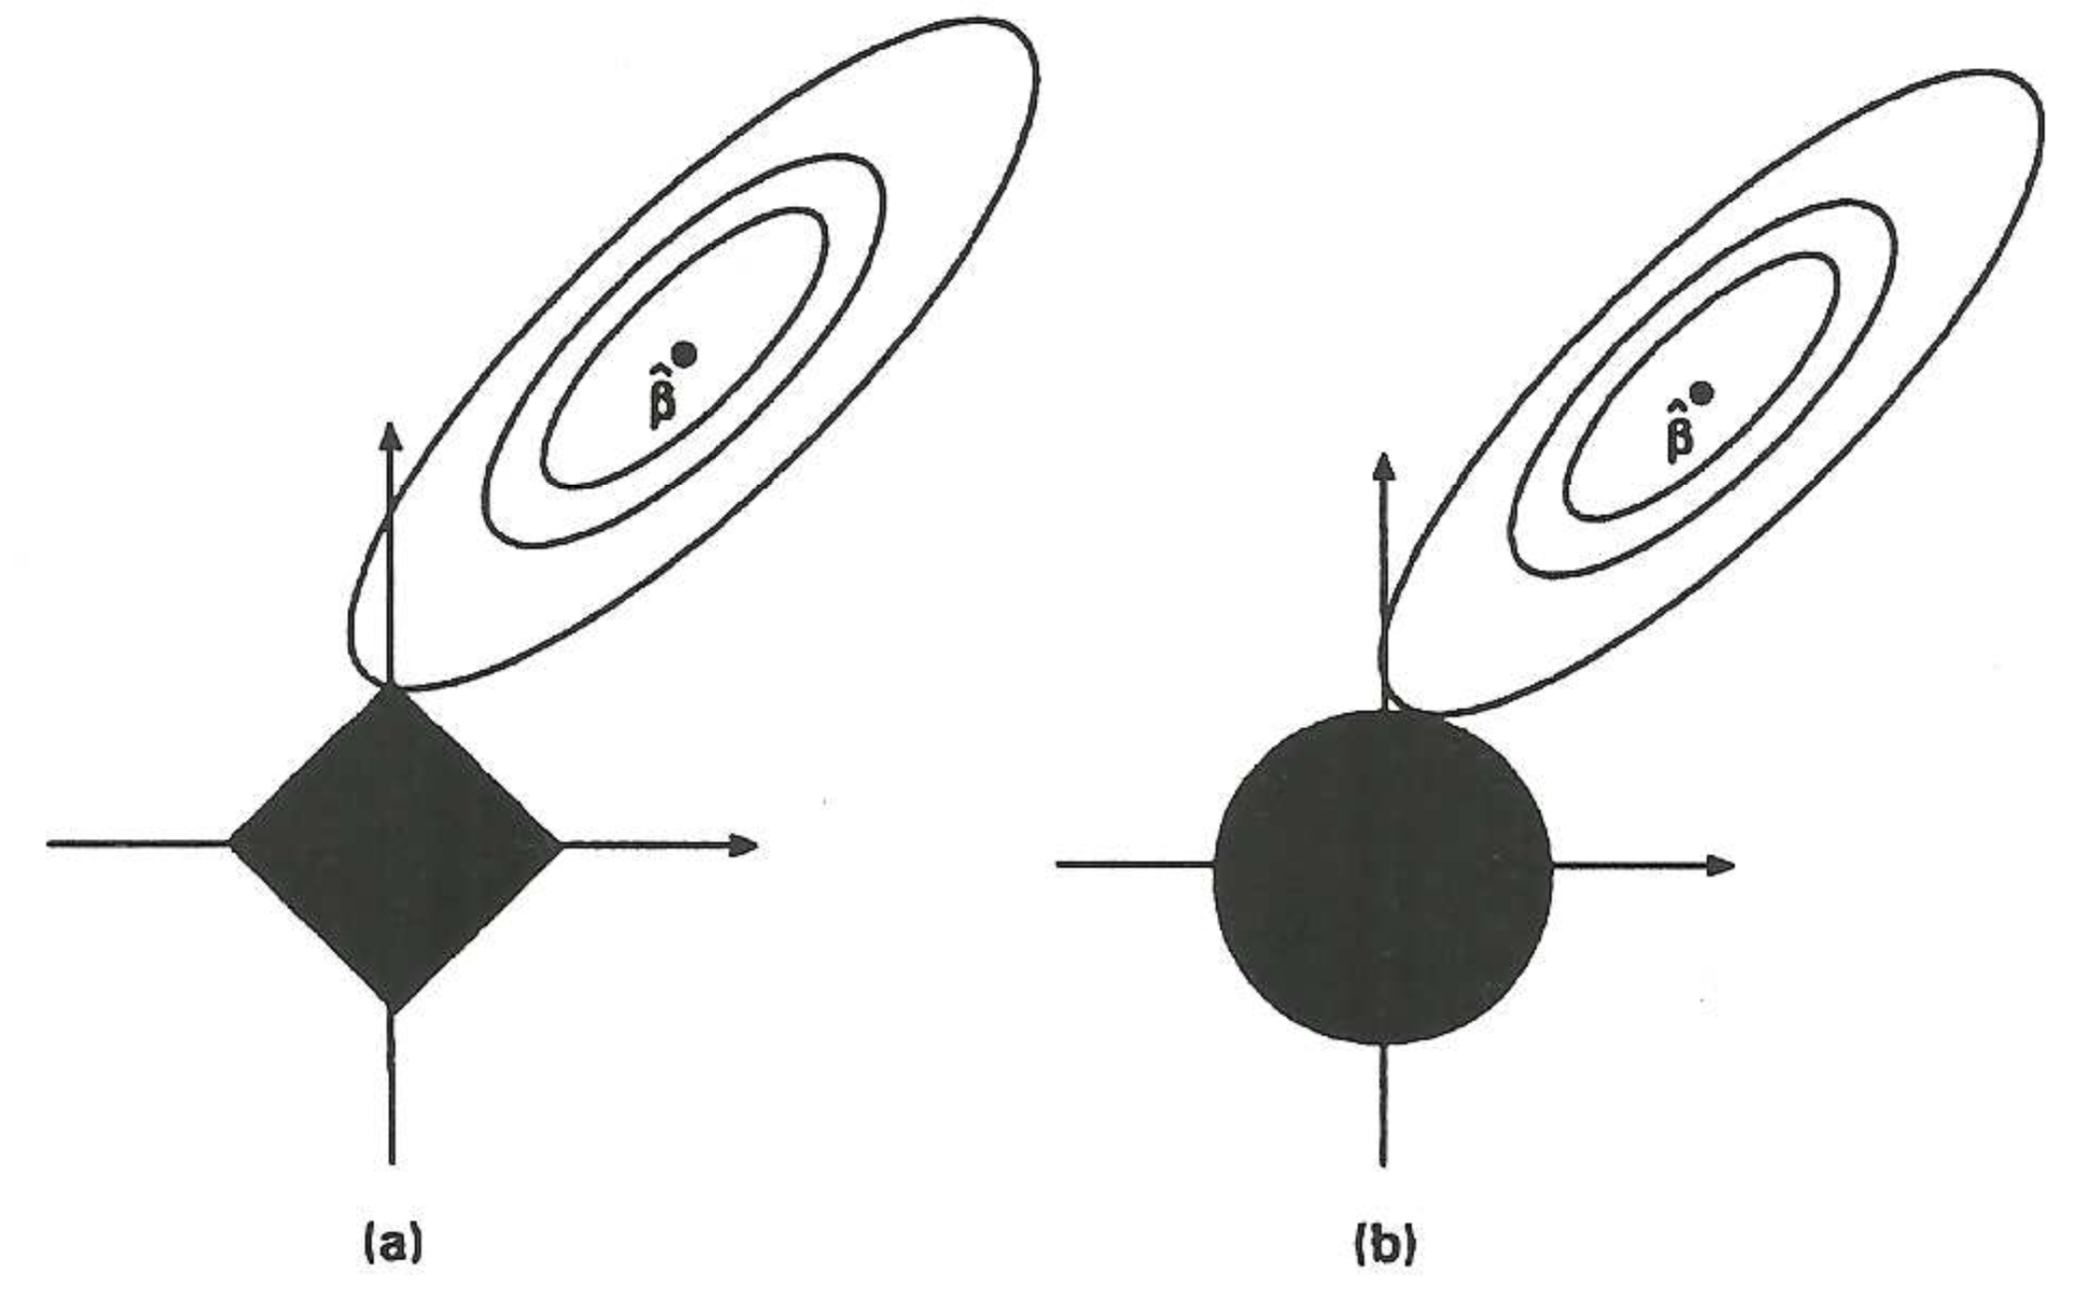
\includegraphics[scale=0.35]{linreg_lasso_level_set.png}
\caption{Level sets of least squares loss function with feasible sets for (a) lasso and (b) ridge regression in the case of \(\beta \in \mathbb{R}^2\).}
\label{linreg.lasso.level.set.figure}
\end{center}
\end{figure}


\subsubsection{Non-Negative Garotte}

This idea inspired the lasso. Proposed by \citet{Breiman1995}. It minimizes

\[
\sum_{i=1}^n \left(y_i - \alpha - \sum_{j=1}^p c_j \hat{\beta}_j^o x_{ij} \right)^2 \text{ subject to } c_j \geq 0, \sum_{j=1}^p c_j \leq t
\]

It starts with OLS estimates and shrinks them by non-negative factors whose sum is constrained. It depends on both the sign and magnitude of OLS estimates. In contrast, lasso avoids the explicit use of OLS estimates.

\subsubsection{LARS---Preliminaries and Intuition}\label{lars.prelims}

Intuition: the algorithm takes steps from a model where all coefficients are 0 to the biggest model (the unpenalized OLS model). Covariates are considered from the highest correlation with \(y\) to the least. (The variable most highly correlated with \(y\) is the one at the ``least angle" from \(y\).) Recall the original definition of the lasso estimator:

\begin{equation}\label{linreg.lasso.constrained}
\hat{\beta}_{lasso} = \underset{\beta \in \mathbb{R}^p}{\arg \min}\left\{ \frac{1}{2n}\lVert y - X \beta \rVert_2^2 \right\} \text{ subject to } \lVert \beta \rVert_1 \leq t
\end{equation}

The more common version now:

\begin{equation}\label{linreg.lasso.lagrangian}
\hat{\beta}_{lasso} =\underset{\beta \in \mathbb{R}^p}{\arg \min} \left\{ \frac{1}{2n}\lVert y - X \beta \rVert_2^2   + \lambda \lVert \beta \rVert_1 \right\}
\end{equation}

One form can be changed to the other by applying Lagrangians\footnote{However, the correspondence between \(t\) and \(\lambda\) is \textbf{not} one-to-one. Because with \(t = \infty\), \(\lambda =0\). But a slightly smaller \(t\) would result in the same solution.}. Have to be careful because this is a convex program (quadratic with ``linear" constraint---use a slack variable). 

Taking the gradient of the loss function in (\ref{linreg.lasso.lagrangian}) yields

\[
\nabla \bigg(  \frac{1}{2n}\lVert y - X \beta \rVert_2^2   + \lambda \lVert \beta \rVert_1 \bigg) = \nabla   \bigg( \frac{1}{2n}\lVert y - X \beta \rVert_2^2   \bigg) + \lambda \nabla \big( \lVert \beta \rVert_1 \big)
\]

\begin{equation}\label{linreg.lasso.lagrangian.gradient}
= - \frac{1}{n} X^T(y - X \beta) + \lambda \nabla  \big( \lVert \beta \rVert_1 \big)
\end{equation}

We set this equal to zero. If the first term equals 0, the residual has to equal 0. For the second part to equal zero, we have to account for the fact that the gradient doesn't exist at 0. In the one-dimensional case \(g(t) = |t|\), we have

\[
g'(t) = \begin{cases}
-1 & t < 0 \\
1 & t > 0
\end{cases}
\]

but it doesn't exist at 0. Instead of using the gradient, we will use \(\partial\), the subdifferential, which is the set of all subgradients. We have a solution if 0 is in the subdifferential. We can rewrite (\ref{linreg.lasso.lagrangian.gradient}) using the subdifferential instead of the gradient:

\[
\partial \bigg(  \frac{1}{2n}\lVert y - X \beta \rVert_2^2   + \lambda \lVert \beta \rVert_1 \bigg) = \nabla \bigg(  \frac{1}{2n}\lVert y - X \beta \rVert_2^2  \bigg)  + \lambda \partial \big( \lVert \beta \rVert_1 \big)  =  - \frac{1}{n} X^T(y - X \beta) + \lambda \partial \big( \lVert \beta \rVert_1 \big)
\]

Then rather than setting the gradient equal to 0, our condition is

\[
0 \in - \frac{1}{n} X^T(y - X \beta) + \lambda \partial \big( \lVert \beta \rVert_1 \big)
\]

Note that 

\[
\partial g (t) = \begin{cases}
-1 & t < 0 \\
[-1, 1] & t = 0 \\
1 & t > 0
\end{cases} = \begin{cases}
\operatorname{sgn}(t) & t \neq 0 \\
[-1, 1] & t = 0 
\end{cases}
\]

so we have

\begin{equation}\label{linreg.lasso.soln.cond}
0 \in - \frac{1}{n} X^T(y - X \beta) + \lambda \cdot \begin{bmatrix} \begin{cases}
\operatorname{sgn}(\beta_j) & t \neq 0 \\
[-1, 1] & \beta_j = 0 
\end{cases} \end{bmatrix}
\end{equation}

where 

\[
\begin{bmatrix} \begin{cases}
\operatorname{sgn}(\beta_j) & t \neq 0 \\
[-1, 1] & \beta_j = 0 
\end{cases} \end{bmatrix} \in \mathbb{R}^p
\]

is a vector with each entry as specified.

\begin{remark}
\begin{enumerate}[(1)]
\item Examining the \(j\)th component of the separable equation (\ref{linreg.lasso.soln.cond}), if \(\beta_j \neq 0\), we have

\[
0 = -\frac{1}{n} X_j^T(y - X \beta) + \lambda \cdot
\operatorname{sgn}(\beta_j) \iff \frac{1}{n} X_j^T(y - X \beta) = \lambda \cdot
\operatorname{sgn}(\beta_j) 
\]

Note that the left side contains the correlation between \(X_j\) and \(e = y - X \beta\), the residual vector. \textbf{So if lasso chooses \(k\) variables, all \(k\) of them will have the same correlation with the residual (\(\lambda\)).}

\item If \(\beta_j =0\), we have

\[
0 \in - \frac{1}{n} X^T(y - X \beta) + \lambda \cdot 
[-1, 1]  \iff \left|  \frac{1}{n} X^T(y - X \beta)  \right| \leq \lambda
\]

\textbf{So for unselected features, the (absolute) correlation should be bounded by \(\lambda\).}

\end{enumerate}

\end{remark}

These two conditions relate to the KKT conditions (first order conditions).

So if we start with \(\lambda\) very large and gradually decrease it, we will let in as the first feature the one that is most highly correlated with \(y\)---that is, the feature with the \textit{least angle} between it and \(y\).


\subsubsection{LARS}

\begin{figure}
\center{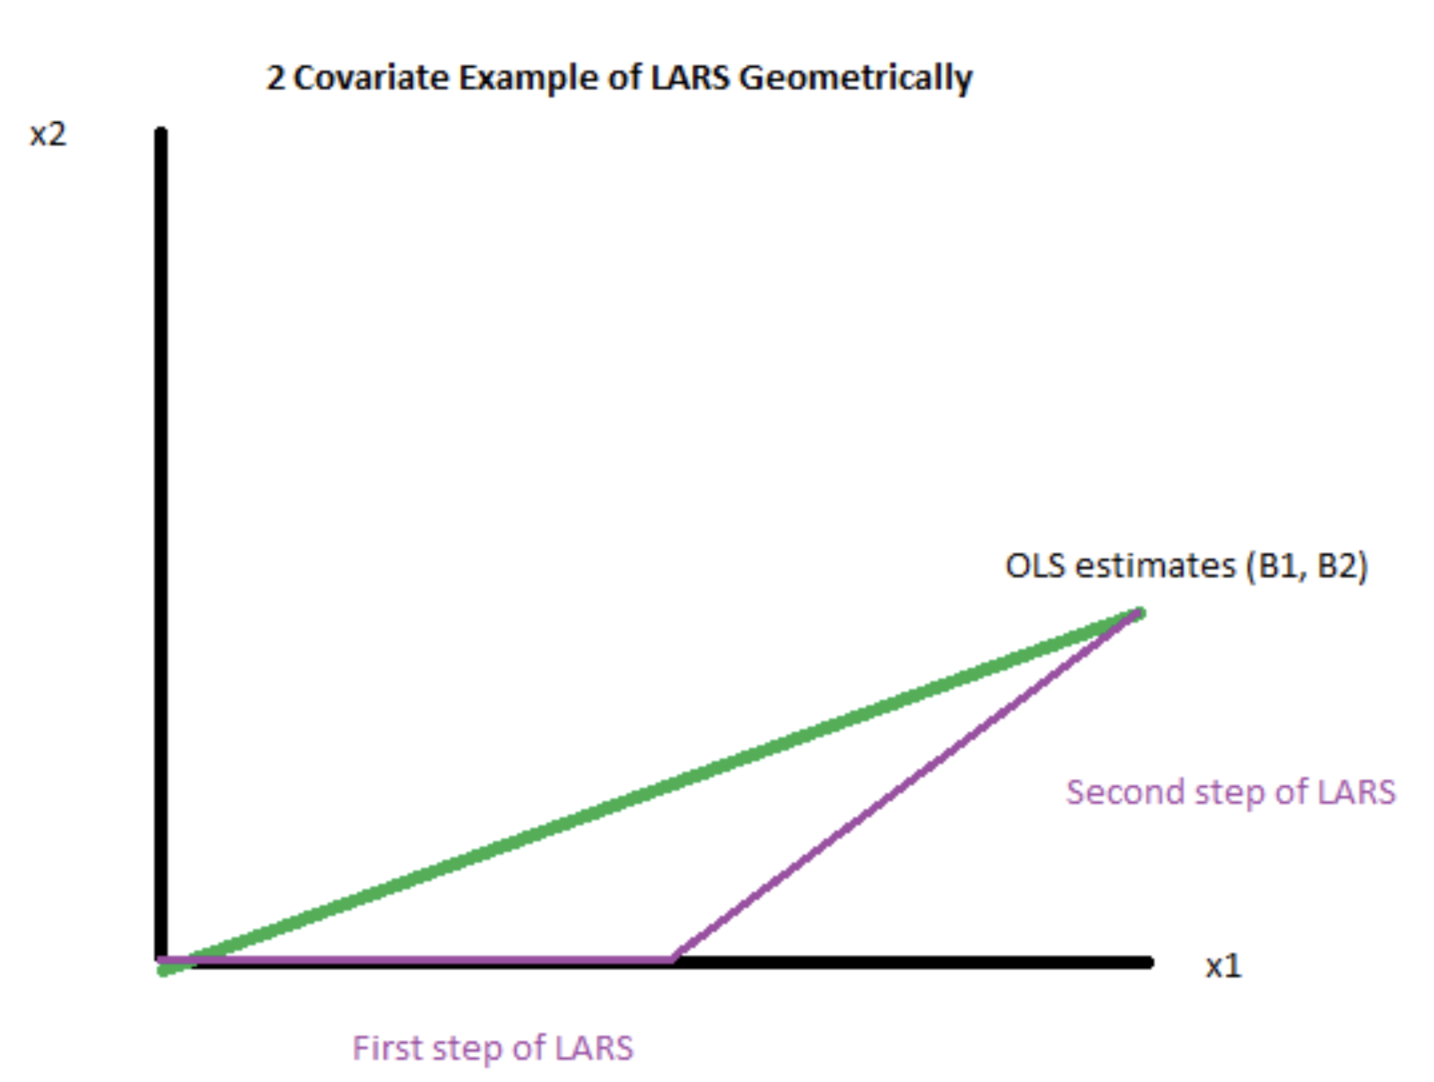
\includegraphics[width=0.8\textwidth, angle=0]{linreg_lars_2d.png}}
\caption{\label{fig:lars_2d} LARS figure in 2d case.}
\end{figure}

\begin{figure}
\center{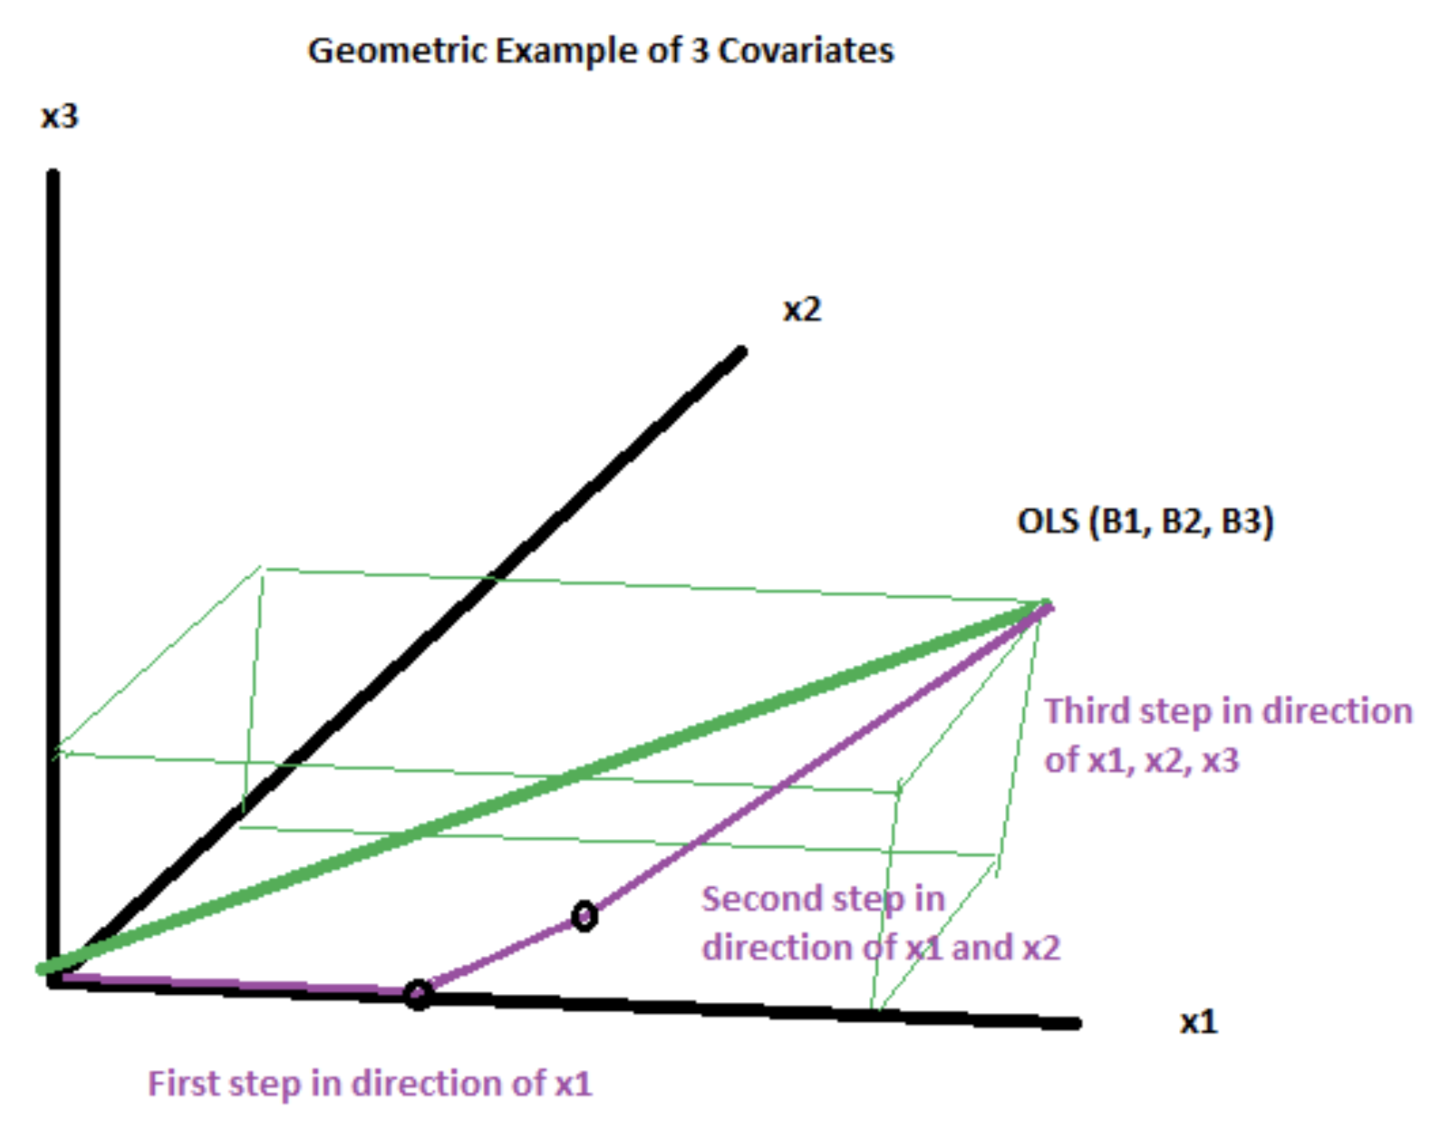
\includegraphics[width=0.8\textwidth, angle=0]{linreg_lars_3d.png}}
\caption{\label{fig:lars_3d} LARS figure in 3d case.}
\end{figure}

In Figure \ref{fig:lars_2d}, note that we choose feature \(X_1\) first because it has the highest correlation with \(y\). As the coefficient on \(X_1\) increases, the correlation between \(X_1\) and the residual with \(y\) decreases, while the correlation between \(X_2\) and the residual remains constant (\textbf{increases?}). When the correlation between \(X_1\) and the residual becomes equal to the correlation between \(X_2\) and the residual, \(X_2\) enters the lasso path.

\begin{remark} Just like in lasso, in LARS the correlation between all included features and the residual are equal (see the remark in Section \ref{lars.prelims}). However, LARS is a stepwise procedure---once we add a feature, it stays in the model. In the lasso, features can be dropped later in the path after they are selected---whenever \(\beta_j\) becomes 0, it is dropped from the current active set. A feature's sign cannot change in lasso---it is not possible. If we modify the LARS algorithm to have this property (``lasso modification"), then the result is the lasso estimator.

\end{remark}

The LARS algorithm for lasso has order \(\mathcal{O}(np \cdot \min \{n, p\})\). In particular, if \(p > n\) it has order \(\mathcal{O}(n^2p)\).


\subsection{Quadratic Loss}

\begin{theorem}\label{exercise6.5}
Let $X:\Omega\to\mathbb{R}$ be a random variable with $\E X^{2}<\infty$. Then $\E(X-t)^{2}$ is minimized for $t\in\mathbb{R}$ uniquely when $t=\E X$.
\end{theorem}

\begin{proof}

%\textbf{proof definitely in Mostly Harmless Econometrics but might be less rigorous, possibly in Pesaran book, possible in stats 100C course notes.}

We seek

\[
 \arg \min_t \E(X - t)^2 = \arg \min_t \big[ \E(X^2) - 2t\E(X) + t^2 \big] = \arg \min_t \big[  t^2 - 2t\E(X)\big] 
\]

where the last step follows because \(\E(X^2)\) is independent of \(t\). This expression is quadratic in \(t\). Differentiating with respect to \(t\) and setting equal to 0, we have

\[
2t - 2 \E(X) = 0 \implies \boxed{\arg \min_t \E(X - t)^2 = \E(X)}
\]

\end{proof}

\subsubsection{Feature Selection properties}

Model selection consistency: \(\Pr(\operatorname{supp}(\hat{\beta}) = \operatorname{supp}(\beta_0) ) \to 1\).

Oracle property: model selection consistency, asymptotic efficiency as efficient as if true model were known (``efficiency" having to do with the variance given \(n\)).

\begin{definition}[\textbf{Oracle property}] Let \(\beta^0\) denote the true parameter vector for data generated from a linear model. Let \(S_0\) be the true support; that is, \(S_0 = \{j: \beta_j^0 \neq 0, j = 1, \ldots, p\}\). Denote \(\hat{\beta}(\delta)\) the coefficient estimator for fitting procedure \(\delta\). We call \(\delta\) an \textbf{oracle procedure} if \(\hat{\beta}(\delta)\) asymptotically has the following properties:

\begin{itemize}

\item Identifies the right subset model (consistency): \(\{j: \hat{\beta}_j \neq 0\} = S_0\).

\item Has the optimal estimation rate: \(\sqrt{n}(\hat{\beta}(\delta)_{S_0} - \beta_{S_0}^0) \xrightarrow{d} \mathcal{N}(0, \Sigma_0)\) where \(\Sigma_0\) is the covariance matrix knowing the true subset model.

\end{itemize}

\end{definition}

The lasso problem is convex but not necessarily strictly convex if \(p > n\). That is, there is some flat region, so the minimizer may not be unique. Consider the KKT conditions from convex optimization:

\[
g(\beta) = \arg \min \left\{ \frac{1}{2n} \lVert y - X \beta \rVert_2^2 + \lambda \lVert \beta \rVert_1 \right\} =  \arg \min \left\{ f_1(\beta) + f_2(\beta) \right\}
\]

Then \(\hat{\beta}\) is a lasso solution if and only if 0 is in the subdifferential of \(g(\hat{\beta})\). Note that 

\[
\partial g(\hat{\beta}) = \nabla f_1 + \partial f_2 = \frac{1}{n} X^T(X \beta - y) + \lambda \begin{bmatrix}  \vdots \\ \partial | \beta_j | \\ \vdots \end{bmatrix} = \frac{1}{n} X^T(X \beta - y) + \lambda \begin{bmatrix}  \vdots \\ \begin{cases}  \operatorname{sgn}(\beta_j) & \beta_j \neq 0 \\ [-1, 1] & \beta_j = 0 \end{cases} \\ \vdots \end{bmatrix}
\]

Now assume \(\operatorname{supp}(\hat{\beta}) = \operatorname{supp}(\beta_0)\) (that is, assume lasso recovers the correct support). Suppose the first \(s\) features are nonzero and consider one of them (so we know that we should have \(\hat{\beta_j} \neq 0\)):

\[
0 \in \partial g(\hat{\beta}) \implies 0 \in \partial_j g(\hat{\beta}) = \bigg[ \frac{1}{n} X^T(X \beta - y) \bigg]_j + \lambda \operatorname{sgn}(\hat{\beta}_j) 
\]

Therefore

\begin{equation}\label{linreg.lasso.first.cond}
\frac{1}{n} X_A^T(X \hat{\beta} - y) + \lambda  \operatorname{sgn}(\hat{\beta}_j) = 0
\end{equation}

where \(X_A\) is a submatrix of \(X\) containing the columns corresponding to the features in the true support, is our first condition. Next, consider what happens for \(j > s\) (features not in the true support). We have

\[
0 \in \partial g(\hat{\beta}) \implies 0 \in \partial_j g(\hat{\beta}) = \bigg[ \frac{1}{n}X^T(X \beta - y) \bigg] + \lambda [-1, 1]
\]

\begin{equation}\label{linreg.lasso.bound.cond}
\implies \left\lVert \frac{1}{n} X_{A^C}^T (X \hat{\beta} - y) \right\rVert_\infty \leq \lambda
\end{equation}

where \(X_{A^C}\) is a submatrix of \(X\) containing the columns corresponding to the features not in the true support, is our boundary condition. Recall the true model

\[
y = X \beta_0 + \epsilon
\]

and consider the case \(X = \begin{bmatrix}X_1 & X_2 \end{bmatrix}\) where \(X_1\) are the features in the true model and \(X_2\) are noise features; that is, \(\beta_0 = \begin{bmatrix} \beta_1 \\ 0 \end{bmatrix}\). Then we are assuming

\[
\hat{\beta}_{\text{lasso}} = \begin{bmatrix} \hat{\beta_1} \\ 0 \end{bmatrix}.
\]

We have from (\ref{linreg.lasso.first.cond})

\[
0 = \frac{1}{n} X_1^T(X \hat{\beta} - y) + \lambda  \operatorname{sgn}(\hat{\beta}_1) = \frac{1}{n} X_1^T(X_1 \hat{\beta}_1 - X_1 \beta_1 - \epsilon) + \lambda  \operatorname{sgn}(\hat{\beta}_1) 
\]
% = \frac{1}{n}(  X_1^TX_1 \hat{\beta}_1 - X_1^TX_1 \beta_1 - X_1^T \epsilon) + \lambda  \operatorname{sgn}(\hat{\beta}_1)
\[
 \iff \frac{1}{n} X_1^TX_1 (\hat{\beta}_1 - \beta_1)  =  \frac{1}{n} X_1^T \epsilon - \lambda  \operatorname{sgn}(\hat{\beta}_1)
 \]
 
 Let's assume that \(\operatorname{sgn}(\hat{\beta}) = \operatorname{sgn}(\beta_0)\) (sign consistency).
 
 \[
  \iff \frac{1}{n} X_1^TX_1 (\hat{\beta}_1 - \beta_1)  =  \frac{1}{n} X_1^T \epsilon - \lambda  \operatorname{sgn}(\beta_1)
  \]
  
  which is linear in \(\hat{\beta}\). Solving, we have
  
\begin{equation}\label{linreg.lasso.first.cond.solved}
  \iff  \hat{\beta}_1 - \beta_1  =  ( X_1^TX_1)^{-1} \big( X_1^T \epsilon - n  \lambda  \operatorname{sgn}(\beta_1)\big)   \iff  \hat{\beta}_1   = \beta_1 +   ( n^{-1}X_1^TX_1)^{-1} \big( n^{-1} X_1^T \epsilon -   \lambda  \operatorname{sgn}(\beta_1) \big)
\end{equation}

Looking at the second (boundary) condition (\ref{linreg.lasso.bound.cond}), we have

\begin{equation}\label{linreg.lasso.bound.cond.cont}
\left\lVert \frac{1}{n} X_{2}^T (X \hat{\beta} - y) \right\rVert_\infty \leq \lambda.
\end{equation}

Consider that 

\[
X \hat{\beta}- y = X_1 \hat{\beta}_1 - X_1 \beta_1 - \epsilon = X_1(\hat{\beta}_1 - \beta_1) - \epsilon
\]

Substituting in the result from (\ref{linreg.lasso.first.cond.solved}) yields

\[
X \hat{\beta}- y  = X_1\big[  ( n^{-1} X_1^TX_1)^{-1} \big( n^{-1} X_1^T \epsilon -  \lambda  \operatorname{sgn}(\beta_1)\big)   \big] - \epsilon
\]

which when we plug into (\ref{linreg.lasso.bound.cond.cont}) yields

\[
\left\lVert \frac{1}{n} X_{2}^T \left[X_1  (n^{-1} X_1^TX_1)^{-1} \big( n^{-1} X_1^T \epsilon -  \lambda  \operatorname{sgn}(\beta_1)\big) - \epsilon\right] \right\rVert_\infty \leq \lambda.
\]

\[
\iff \left\lVert \frac{1}{n} X_{2}^T X_1 (n^{-1} X_1^TX_1)^{-1} \big( n^{-1} X_1^T \epsilon -  \lambda  \operatorname{sgn}(\beta_1)\big)    -  \frac{1}{n} X_{2}^T \epsilon \right\rVert_\infty \leq \lambda.
\]

Using the Triangle Inequality, we have

\[
\left\lVert \frac{1}{n} X_{2}^T X_1 (n^{-1} X_1^TX_1)^{-1} \big( n^{-1} X_1^T \epsilon -  \lambda  \operatorname{sgn}(\beta_1)\big)    -  \frac{1}{n} X_{2}^T \epsilon \right\rVert_\infty 
\]

\[
\leq \left\lVert \frac{1}{n} X_{2}^T X_1 (n^{-1} X_1^TX_1)^{-1} \big( n^{-1} X_1^T \epsilon -  \lambda  \operatorname{sgn}(\beta_1)\big)  \right\rVert_\infty + \left\lVert  \frac{1}{n} X_{2}^T \epsilon \right\rVert_\infty 
\]

\begin{equation}\label{linreg.lasso.bound.cond.cont.more}
\leq \left\lVert \frac{1}{n} X_{2}^T  X_1 (n^{-1} X_1^TX_1)^{-1} \right\rVert_\infty \cdot \left\lVert  n^{-1} X_1^T \epsilon -  \lambda  \operatorname{sgn}(\beta_1)    \right\rVert_\infty + \left\lVert  \frac{1}{n} X_{2}^T \epsilon \right\rVert_\infty 
\end{equation}

Assume that the \(j\)th column of \(X\) has \(L_2\) norm \(n^{1/2}\) (as it would if all entries equaled 1). We have

\[
\left\lVert n^{-1} X_1^T \epsilon \right\rVert_\infty \leq \lambda/2, \qquad \left\lVert n^{-1} X_2^T \epsilon \right\rVert_\infty \leq \lambda/2
\]

\[
\left\lVert n^{-1} X^T \epsilon \right\rVert_\infty \leq \lambda/2 \text{ with large probability}
\]

Recall that \(\lambda = \sigma \sqrt{ \frac{c \log p }{n} } \) for some \(c >2\). Then we have (continuing from (\ref{linreg.lasso.bound.cond.cont.more})), and using \( \left\lVert n^{-1}X_2^T \epsilon \right\rVert \leq \lambda/2\), 

\[
\leq \left\lVert n^{-1} X_1^T \epsilon \right\rVert_\infty + \left\lVert \lambda \operatorname{sgn}(\beta_1)   \right\rVert_\infty
\]

\[
 \left\lVert n^{-1} X_2^T X_1(n^{-1}X_1^T X_1)^{-1} \right\rVert_\infty \cdot \underbrace{ \left\lVert \cdot \right\rVert_\infty}_{3/2 \lambda} + \underbrace{\left\lVert \cdot \right\rVert_\infty}_{\lambda/2} \leq \lambda
\]

\begin{equation}\label{linreg.lasso.irrep}
 \left\lVert \underbrace{n^{-1} X_2^T X_1}_{\text{corr. between noise and true}}( \underbrace{n^{-1}X_1^T X_1}_{\text{sample covariance matrix}})^{-1} \right\rVert_\infty  \leq 1/3
\end{equation}

It turns out we're fine as long as it's less than or equal to 1. This is known as the \textbf{irrepresentable condition}. Note that the sample covariance matrix is the same as the sample correlation since the columns are standardized. So this is the correlation between the true variables. Note that this matrix has dimension \((p-s) \times s\) where \(s\) is the dimension of the true support. Note that

\[
n^{-1} X_2^T X_1( n^{-1}X_1^T X_1)^{-1} = (X_2^T X_1 (X_1^T X_1)^{-1}]^T =(X_1^T X_1)^T X_1^T X_2
 \]
 
which is ordinary least squares for regressing \(X_2\) on \(X_1\). In the end, the irrepresentable condition says the correlation between the noise and true variables can't be too high.

\subsection{Dantzig Selector}

Dantzig selector:

%\[
%\min_{\beta \in \mathbb{R}^p} \lVert \beta \right\rVert_1 \text{ s.t. } \lVert n^{-1} X^t(y - X \beta) \right\rVert_\infty \leq \lambda
%\]

\[
\begin{aligned}
\hat{\beta}_{\text{Dantzig}}  =  & {\underset {\beta \in \mathbb{R}^p}{\arg \min}}
& &  \lVert \beta \rVert_1 \\
& \text{subject to}
& &  \lVert n^{-1} X^T(y - X \beta) \rVert_\infty \leq \lambda
\end{aligned}
\]

Can be recast as a linear program:

\begin{equation}\label{linreg.dantzig.lp}
\begin{aligned}
\hat{\beta}_{\text{Dantzig}} =  & {\underset {u \in \mathbb{R}^p}{\arg \min}}
& & \sum_{i=1}^p u_i  \\
& \text{subject to}
& & -u \leq \beta \leq u \\
& & & -\lambda_p \sigma \boldsymbol{1} \leq n^{-1} X^T(y - X \beta) \leq \lambda_p \sigma \boldsymbol{1}
\end{aligned}
\end{equation}

where \(|u|\) denotes the absolute value of \(u\) componentwise. (This is a benefit because linear programming is easy to use and very popular in industry and other applications.) Note that \( n^{-1} X^t(y - X \beta) \) corresponds to the correlations between the residuals and the design matrix. Recall that in OLS this correlation is 0---the design matrix is orthogonal to the residuals. In the Dantzig selector we relax this, bounding the \(L_\infty\) norm by \(\lambda\). Recall that the gradient of the log-likelihood is the \textbf{score function}, in this case \(n^{-1} X6t(y - X \beta)\). For example, the score equation in linear regression is \(n^{-1} X^Ty = n^{-1} X^T X \beta\). Note:

\[
 \nabla \bigg( \frac{1}{2n} \lVert y - X \beta \rVert_2^2  \bigg) = \frac{1}{n} X^T (X \beta - y)
\]

Note for Theorem 1: in original paper, assumed columns had \(L_2\) norm 1, resulting in \(\lambda_p = \sqrt{2 \log p}\). We are instead assuming each column has \(L_2\) norm \(\sqrt{n}\), which results in \(\lambda = \sigma \cdot \sqrt{\frac{c \log p}{n}}\). Intuition of \(\log p\) term: 


By a theorem in \citet{James2009}, the lasso and Dantzig selector estimates equal each other under certain conditions:

\begin{theorem}\label{linreg.lasso.dantzig.thm1} Let \(I_l\) be the support of the lasso estimate \(\hat{\beta}_{\text{lasso}}\). Let \(\boldsymbol{X}_L\) be the \(n \times | I_L|\) matrix constructed by taking \(\boldsymbol{X}_{I_L}\) and multiplying its columns by the signs of the corresponding coefficients in \(\hat{\beta}_{\text{lasso}}\). Suppose that \(\lambda_{\text{lasso}} = \lambda_{\text{Dantzig}}\). Then \(\hat{\beta}_{\text{lasso}} = \hat{\beta}_{\text{Dantzig}}\) if \(\boldsymbol{X}_L\) has full rank and 

\[
\boldsymbol{u} = \big( \boldsymbol{X}_L^T \boldsymbol{X}_L \big)^{-1} \boldsymbol{1} \succeq 0 \text{ and } \lVert \boldsymbol{X}^T \boldsymbol{X}_L \boldsymbol{u} \rVert_\infty \leq 1
\]

where \(\boldsymbol{1} \) is an \(| I_L|\)-vector of ones and the vector inequality is understood componentwise.

\end{theorem}

\begin{corollary} If \(\boldsymbol{X}\) is orthonormal (\(\boldsymbol{X}^T \boldsymbol{X} = \boldsymbol{I}_p\)), then the entire lasso and Dantzig selector coefficient paths are identical.

\end{corollary}

\begin{proof} For each index set \(\boldsymbol{I}\), \(\boldsymbol{X}^T \boldsymbol{X} = \boldsymbol{I}_{| \boldsymbol{I} |}\), so clearly both of the conditions of Theorem \ref{linreg.lasso.dantzig.thm1} are satisfied.

\end{proof}


The entire paths can be identical under another condition presented in the same paper.

\begin{theorem}
Suppose that all pairwise correlations between the columns of \(\boldsymbol{X}\) are equal to the same value \(\rho\) where \(0 \leq \rho < 1\). Then the entire Lasso and Dantzig selector coefficient paths are identical. In addition, when \(p=2\), the same holds for every \(\rho \in (-1, 1)\).

\end{theorem}

\subsection{Coordinate Descent}

Start with \(\beta_1\) varying and all other \(\beta\)s fixed. Optimize \(\beta_1\). Then cycle through each \(\beta_j\), run until convergence.

\subsection{Nonconvex Learning}

\subsection{Yinfei Kong---Innovated Interaction Screening for HIgh-Dimensional Nonlinear Classification}


\subsection{Total Variational Distance}



%
%
%
%
%
%
%
%
%

%\bibliographystyle{abbrvnat}
%\bibliography{mybib2fin}
%\end{document}



